%=============================================================================
% JOE submission — Code-aware joint estimation/detection (JUNA) for
% Doppler-induced ICI in underwater acoustic OFDM.
%
% The equations, the JunaCore package, and the measured ReplayCh workbench are
% three evidence layers. Measured tables below carry accepted benchmark numbers
% from the separate ReplayCh workbench; package constants and controlled WCz
% results are protected by test/walkthrough_contract.jl.
%=============================================================================
\documentclass[journal]{IEEEtran}

\usepackage{amsmath,amssymb,amsfonts}
\usepackage{bm}
\usepackage{graphicx}
\usepackage{booktabs}
\usepackage{array}
\usepackage{algorithm}
\usepackage{algpseudocode}
\usepackage{url}
\usepackage[hidelinks]{hyperref}
\usepackage{cite}
\usepackage{tikz}
\usetikzlibrary{arrows.meta,positioning,fit,backgrounds}

\graphicspath{{../../tex/figure_data/}}

\definecolor{labPanel}{HTML}{F6FBFA}
\definecolor{labLine}{HTML}{28413C}
\definecolor{labTeal}{HTML}{14B8A6}
\definecolor{labTealLight}{HTML}{D7FBF5}
\definecolor{labBlue}{HTML}{4777D9}
\definecolor{labBlueLight}{HTML}{E6EEFF}
\definecolor{labGold}{HTML}{C8871E}
\definecolor{labGoldLight}{HTML}{FFF1D4}
\definecolor{labViolet}{HTML}{7C5CCB}
\definecolor{labVioletLight}{HTML}{EEE7FF}
\definecolor{labGreenLight}{HTML}{DDF7EF}

% --- macros (from gab.tex) ---
\newcommand{\C}{\mathbb{C}}
\newcommand{\R}{\mathbb{R}}
\newcommand{\F}{\mathbb{F}}
\newcommand{\E}{\mathbb{E}}
\newcommand{\Ht}{^{H}}
\newcommand{\T}{^{T}}
\newcommand{\norm}[1]{\left\lVert #1 \right\rVert}
\newcommand{\abs}[1]{\left\lvert #1 \right\rvert}
\newcommand{\cfg}[1]{\texttt{#1}}
\newcommand{\juna}{JUNA}
\newcommand{\junalite}{JUNA-lite}
\newcommand{\junawz}{JUNA-Wz}
\newcommand{\junawcz}{JUNA-WCz}
\newcommand{\Hc}{\mathbf H_{\rm c}}
\newcommand{\Hm}{\mathbf H_{\rm m}}

\begin{document}

\title{Code-Aware Joint Estimation and Detection for Doppler-Induced ICI in
Underwater Acoustic OFDM: Measured-Channel Validation}

\author{Gabriel~Chua~Yu~Han
\thanks{Manuscript submitted \today. The author is with the Acoustic Research
Laboratory (e-mail: chuayuhan1985@gmail.com).}}

\markboth{IEEE Journal of Oceanic Engineering}%
{Chua: Code-Aware Joint Estimation and Detection for UWA OFDM}
\maketitle

%=============================================================================
\begin{abstract}
Residual Doppler makes underwater acoustic OFDM depart from the diagonal
subcarrier model: intercarrier interference appears, and a pilot-only equalizer
can land just outside the decoder's basin of attraction. We present \juna{}
(Joint Unified Nonideality-Aware Algorithm), a code-aware receiver family that
places equalization and LDPC decoding in one coupled objective. The measured
gradient receiver, \junawz{}, freezes the explicit ICI tensor and takes
confidence-weighted descent steps over the partial-FFT combiner and soft bit
latents, with LDPC belief-propagation posteriors providing parity structure and
per-symbol confidence. Unlike path-based or banded-ICI channel-estimation
receivers, \juna{} does not deploy a full frequency-domain ICI-matrix estimator;
that model motivates the update and is exercised separately as a diagnostic. A
lightweight variant, \junalite{}, approximates the same code-aware feedback loop
without explicit gradients---it feeds LDPC posterior means back into the
partial-FFT combiner as posterior-confidence-weighted soft data anchors and
solves a batch ridge-LS refit---recovering most of the gain at a fraction of the
cost. The large measured-channel study was produced by a separate ReplayCh
workbench that implements the same receiver idea with recursive updates. At
20\,dB, \junalite{}+FEC improves packet success over Partial~FFT+FEC in
hard-but-decodable measured channels: from $0.559$ to $0.922$ payload-exact PSR
on the controlled red channel and from $18/190$ to $135/190$ accepted packets on
the hardest native capture, while tying on ceiling channels and failing with the
baselines on floor channels. In stacked head-to-head mirrors, \junawz{} is at
least as good as \junalite{} in $44/48$ capture--SNR cells, has $18$ disjoint
Wilson-interval wins and no disjoint losses, and has four small non-significant
regressions on near-floor NA cells. A
twelve-capture, three-site tuning study shows that FFT size is usually the first
high-impact retuning knob, after which conservative modulation and code-rate
choices keep the receiver inside the decodable regime.
\end{abstract}

\begin{IEEEkeywords}
Underwater acoustic communication, OFDM, intercarrier interference, Doppler,
joint detection and decoding, LDPC, partial-FFT, recursive least squares,
replay channel.
\end{IEEEkeywords}

%=============================================================================
\section{Introduction}\label{sec:intro}
\IEEEPARstart{U}{nderwater} acoustic (UWA) OFDM is attractive because it turns a
long multipath channel into many narrowband subchannels when timing, Doppler
correction, and cyclic-prefix assumptions hold~\cite{li2008nonuniform}. The same
structure becomes fragile when the channel changes over the useful OFDM
interval. Even after packet acquisition and coarse Doppler correction, residual
time variation breaks subcarrier orthogonality, spreads energy into neighboring
bins~\cite{berger2010sparse}, and leaves the receiver with a coupled-carrier
problem rather than a diagonal one.

Partial-FFT demodulation is a serious conventional defense against this
breakdown~\cite{yerramalli2012partialfft}. Instead of representing each
subcarrier by a single FFT coefficient, the receiver slices the OFDM symbol in
time, computes several partial-FFT observations per carrier, and learns a local
linear combiner---here a bandwise combiner trained on known pilots. This
baseline is far stronger than one-tap OFDM; in our
replay workbench it is the strongest non-decoder-feedback receiver. Its
limitation is structural: it trains the equalizer from pilots and only then asks
the LDPC decoder whether the resulting soft symbols make sense. When pilot
support is sparse or the time variation is strong, the pilot-only combiner can
land just outside the decoding basin, even though the decoder posterior often
carries useful global information about the codeword.

\juna{} uses that information before giving up. The formulation treats the
partial-FFT combiner, transmitted data symbols, and code constraints as parts of
one regularized problem. The measured gradient receiver, \junawz{}, uses the
partial-FFT observation vectors and a frozen ICI model, then jointly nudges the
combiner and the soft bit latents toward a configuration consistent with the
pilots and---through the LDPC belief-propagation (BP) posterior---the code. This
is intentionally close in spirit to turbo equalization~\cite{douillard1995turbo,
tuchler2002turbo,jhuang2011progressive}, but architecturally narrower
(Section~\ref{sec:related}): \juna{} does not replace the front end with a
generic soft-in/soft-out equalizer; it keeps the partial-FFT observation
vectors and feeds decoder-weighted information back into that front end. A lightweight variant,
\junalite{}, approximates the same loop without forming any gradient: it maps
the posterior LLRs to posterior-mean constellation points and re-estimates the
same partial-FFT combiner with those means as confidence-weighted soft training
anchors. In the JunaCore reference implementation this is a batch ridge-LS
solve with two refinement passes. The key economy---shared by both---is that a decoded data symbol with a
useful posterior can behave like a \emph{soft pilot}: the LDPC parity graph
supplies structure beyond the physical pilot tones and can share the
equalizer-training burden. Because \junalite{} is cheap enough to run across
every measured capture, it carries the large-scale study, while \junawz{} is
reported on head-to-head mirrors and \junawcz{} remains a diagnostic.

\textbf{Contributions.}
\begin{itemize}
\item A coupled estimation/decoding objective (Section~\ref{sec:juna}) in which
  pilots, partial-FFT observations, the combiner, and the code constraints regularize
  one another.
\item Two bounded receivers derived from it (Section~\ref{sec:solver}):
  \junawz{}, which descends the reduced $(\mathbf W,\mathbf z)$ objective with
  confidence-weighted updates and decoder-grounded checkpoint scoring, and a
  lightweight \junalite{} that approximates the same loop as a
  posterior-anchor batch ridge-LS refit
  (partial-FFT seed $\to$ BP posterior LLRs $\to$ posterior-mean soft data
  anchors $\to$ combiner refit $\to$ candidate selection), with explicit
  anchor-count and iteration limits. The full $(\mathbf W,\mathbf C,\mathbf z)$
  solver, \junawcz{}, is a third public package profile but is reported only in
  controlled and single-segment diagnostics rather than in the measured sweeps.
\item A complexity accounting (Section~\ref{sec:complexity}) that separates the
  online receiver cost from the offline configuration search and quantifies the
  gradient-versus-lite trade.
\item An empirical regime characterization: \juna{} helps in the
  hard-but-decodable regime, ties on ceiling channels, and fails with the
  baselines on floor channels, with \junalite{} carrying the at-scale sweeps and
  \junawz{} tested on head-to-head mirrors.
\item Validation on measured replay captures across three deployment sites
  (Section~\ref{sec:transfer}) and actionable cross-channel tuning guidance.
\end{itemize}

\subsection{Implementation and Evidence Boundary}
This paper distinguishes three related but not identical executables. First,
the equations define the ideal receiver family. Second, the \textbf{JunaCore
reference implementation} in this repository exposes \junalite{}, \junawz{},
and \junawcz{} through one modulation interface and is the source of the
package constants and controlled tests reported below. Third, the
\textbf{separate ReplayCh workbench} produced the measured-channel tables and
figures from replay captures. The ReplayCh code contains related RLS and
prototype solver paths, but those paths are not claimed to be byte-for-byte or
algorithmically identical to JunaCore. Consequently, a JunaCore unit or
round-trip test validates the package implementation; reproducing a measured
table additionally requires the ReplayCh engine, capture data, and generation
scripts named in Section~\ref{sec:method}.

\subsection{Related Work}\label{sec:related}
UWA-OFDM receiver design has largely followed an estimate-then-decode pattern.
One line of work estimates a physical or sparse channel model and derives the
resulting non-diagonal, often locally banded, ICI pattern
explicitly~\cite{berger2010sparse}; another tracks time-varying channels across
blocks by exploiting channel coherence~\cite{zwang2012clustered}. These papers
explain the physical source of the problem studied here, but they are not the
same receiver architecture: they seek explicit channel or ICI estimates, whereas
\junawz{} descends a code-aware reduced objective over an empirical partial-FFT
combiner and the data symbols using decoder-derived confidences (and its
\junalite{}
variant retrains that combiner from decoder-derived soft targets).

Other approaches attack Doppler before this receiver loop by changing the
transmit waveform or the estimation basis. Doppler-resilient orthogonal
signal-division multiplexing (D-OSDM) designs the data/pilot vector layout so
that, under a basis-expansion model of the doubly spread channel, the block
structure is preserved after propagation and Doppler-induced coupling can be
inverted at the receiver~\cite{ebihara2016dosdm}. A second group changes the
observation or estimation basis rather than the modulation: frequency-domain
oversampling of zero-padded OFDM sharpens channel/ICI estimation and reduces
sensitivity to Doppler leakage without altering the transmit
waveform~\cite{wang2012fdoversampling}, and wavelet/filter-bank representations
have been used to refine channel estimation under Doppler
spread~\cite{tang2018haarwavelet}. These methods share \juna{}'s
motivation---all respond to the same Doppler-created off-diagonal coupling---but
move the remedy into the transmit waveform or an alternative channel-estimation
basis. \juna{} instead keeps the measured CP-OFDM/Partial-FFT front end and asks
whether decoder posterior structure can supply additional soft anchors once
residual coupling has already reached the receiver.

Partial-FFT demodulation~\cite{yerramalli2012partialfft} attacks intra-symbol
time variation directly and is the front end we adopt. It replaces one FFT
coefficient per carrier with several time-windowed partial-FFT observations and learns a
linear combiner from pilots. \juna{} keeps this observation-vector representation; the new
step is to let the decoder posterior either weight a reduced gradient update of
the combiner and the soft data symbols (\junawz{}) or provide soft targets for a
bounded anchored ridge-LS refit (\junalite{}). Pilot-aided ICI mitigation outside UWA
similarly motivates the diagonal-to-coupled transition~\cite{mostofi2005ici},
but does not provide this decoder-aided partial-FFT retraining loop.

The closest algorithmic relatives are iterative, turbo-principle ICI receivers
for time-varying UWA channels~\cite{jhuang2011progressive,jhuang2010iterative}.
They exchange extrinsic LLRs between an ICI-cancelling equalizer and the decoder.
\juna{} makes a narrower exchange: decoder confidences \emph{weight} the
\junawz{} update of the partial-FFT combiner and soft data symbols---and, in the
\junalite{} variant, convert decoder \emph{posterior means} into soft data
pilots that retrain the linear combiner---under anchor/iteration caps, optional
confidence thresholding, and decoder-grounded candidate selection. A
broader family of iterative UWA-OFDM receivers couples detection with external
interference cancellation~\cite{zwang2012partialband}, physical-layer network
coding at a relay~\cite{zwang2013plnc}, or asynchronous multiuser
reception~\cite{zwang2013async}; these solve different interference or network
problems. To our knowledge no prior UWA-OFDM receiver feeds decoder posteriors
back into the partial-FFT combiner as soft anchors in this way.

The experiments below therefore make a deliberately narrower comparison: they
isolate the incremental value of posterior-anchor retraining over the one-tap
and partial-FFT receiver variants available in the replay workbench. We do not
claim an empirical win over full turbo ICI cancellers or path-explicit ICI
estimators; implementing those receivers on the same measured captures is an
important but separate comparison. Fig.~\ref{fig:method-comparison} summarizes
the architectural distinction.

\begin{figure*}[t]
\centering
\scriptsize
\resizebox{0.98\textwidth}{!}{%
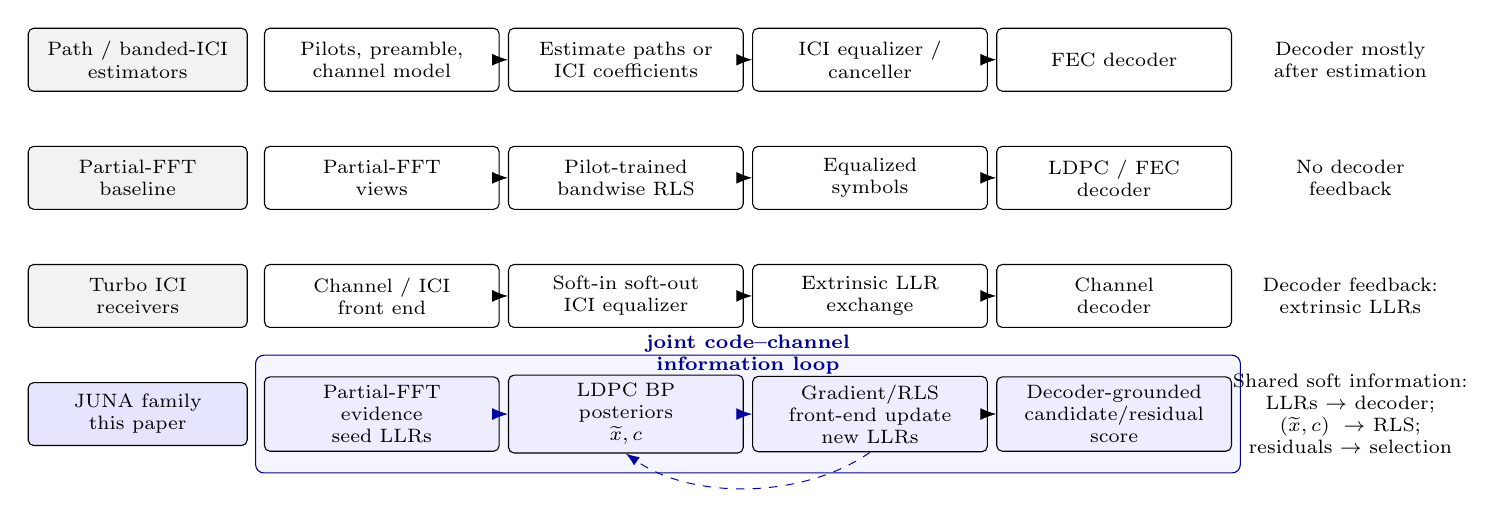
\begin{tikzpicture}[
  font=\scriptsize,
  lane/.style={draw, rounded corners=2pt, align=center, inner xsep=4pt,
    inner ysep=3pt, minimum height=8mm, text width=25mm, fill=gray!10},
  block/.style={draw, rounded corners=2pt, align=center, inner xsep=4pt,
    inner ysep=3pt, minimum height=8mm, text width=27mm, fill=white},
  ours/.style={draw, rounded corners=2pt, align=center, inner xsep=4pt,
    inner ysep=3pt, minimum height=8mm, text width=27mm, fill=blue!7},
  note/.style={align=center, text width=31mm},
  arr/.style={-{Latex[length=2mm]}, line width=0.35pt},
  info/.style={-{Latex[length=1.7mm]}, dashed, blue!65!black,
    line width=0.35pt},
  joint/.style={draw=blue!60!black, fill=blue!4, rounded corners=3pt,
    inner xsep=3pt, inner ysep=7pt}
]
\node[lane] (m1) at (0,3.6) {Path / banded-ICI\\estimators};
\node[block] (a1) at (3.1,3.6) {Pilots, preamble,\\channel model};
\node[block] (b1) at (6.2,3.6) {Estimate paths or\\ICI coefficients};
\node[block] (c1) at (9.3,3.6) {ICI equalizer /\\canceller};
\node[block] (d1) at (12.4,3.6) {FEC decoder};
\node[note] at (15.4,3.6) {Decoder mostly\\after estimation};

\node[lane] (m2) at (0,2.1) {Partial-FFT\\baseline};
\node[block] (a2) at (3.1,2.1) {Partial-FFT\\views};
\node[block] (b2) at (6.2,2.1) {Pilot-trained\\bandwise RLS};
\node[block] (c2) at (9.3,2.1) {Equalized\\symbols};
\node[block] (d2) at (12.4,2.1) {LDPC / FEC\\decoder};
\node[note] at (15.4,2.1) {No decoder\\feedback};

\node[lane] (m3) at (0,0.6) {Turbo ICI\\receivers};
\node[block] (a3) at (3.1,0.6) {Channel / ICI\\front end};
\node[block] (b3) at (6.2,0.6) {Soft-in soft-out\\ICI equalizer};
\node[block] (c3) at (9.3,0.6) {Extrinsic LLR\\exchange};
\node[block] (d3) at (12.4,0.6) {Channel\\decoder};
\node[note] at (15.4,0.6) {Decoder feedback:\\extrinsic LLRs};

\node[lane, fill=blue!10] (m4) at (0,-0.9) {\juna{} family\\this paper};
\node[ours] (a4) at (3.1,-0.9) {Partial-FFT\\evidence\\seed LLRs};
\node[ours] (b4) at (6.2,-0.9) {LDPC BP\\posteriors\\$\widetilde x,c$};
\node[ours] (c4) at (9.3,-0.9) {Gradient/RLS\\front-end update\\new LLRs};
\node[ours] (d4) at (12.4,-0.9) {Decoder-grounded\\candidate/residual score};
\node[note] at (15.4,-0.9) {Shared soft information:\\LLRs $\to$ decoder;\\$(\widetilde x,c)\to$ RLS;\\residuals $\to$ selection};

\begin{scope}[on background layer]
\node[joint, fit=(a4) (b4) (c4) (d4)] {};
\end{scope}
\node[blue!60!black, font=\scriptsize\bfseries, align=center]
  at (7.75,-0.15) {joint code--channel\\information loop};

\foreach \s/\t in {a1/b1,b1/c1,c1/d1,a2/b2,b2/c2,c2/d2,a3/b3,b3/c3,c3/d3,c4/d4}
  \draw[arr] (\s) -- (\t);
\draw[arr, blue!65!black] (a4) -- (b4);
\draw[arr, blue!65!black] (b4) -- (c4);
\draw[info] (c4.south) to[out=-145,in=-35,looseness=0.85]
  (b4.south);
\end{tikzpicture}%
}
\caption{Receiver information-flow comparison. Path-explicit and banded-ICI
methods estimate channel/ICI coefficients before decoding; the Partial-FFT
baseline trains a partial-FFT combiner only from pilots; turbo ICI receivers exchange
extrinsic LLRs with a soft equalizer; the \juna{} family keeps the Partial-FFT
front end and closes the shaded joint code--channel loop by sharing soft
information. Partial-FFT observation-vector evidence produces seed LLRs, LDPC BP returns
posterior means and confidences, \junawz{} uses them in a reduced gradient update
while \junalite{} uses them as RLS soft anchors, and updated LLRs/residual
evidence return to the decoder without deploying a full ICI-matrix estimator.}
\label{fig:method-comparison}
\end{figure*}

%=============================================================================
\section{OFDM Under Residual Doppler}\label{sec:model}
\subsection{Diagonal CP-OFDM}
Consider one OFDM symbol with $N$ subcarriers, cyclic prefix (CP) length
$N_{\mathrm{cp}}$, pilot set $\mathcal P$, data set $\mathcal D$, and unitary DFT
matrix $\mathbf F$. Let $\mathbf X\in\C^N$ be the transmitted frequency-domain
symbol and $\mathbf x=\mathbf F\Ht\mathbf X$ its time-domain block. If the
channel is $L$-tap, time invariant over the block, and $L-1\le N_{\mathrm{cp}}$,
CP removal yields a circulant model and, after the FFT,
\begin{equation}
  \mathbf Y=\mathbf F\mathbf H_{\mathrm{cir}}\mathbf F\Ht\mathbf X+\bm\nu
  =\operatorname{diag}(\mathbf H)\mathbf X+\bm\nu,
  \label{eq:diagonal-ofdm}
\end{equation}
so each carrier obeys the one-tap model $Y_k=H_kX_k+\nu_k$, and pilot-linear
equalization estimates $H_k$ on pilots and interpolates.

\subsection{Residual Doppler and Non-Diagonal Coupling}
Under Doppler the received packet is time-scaled, $r(t)=s\big((1+a)t\big)$, with
$a$ the residual scale after coarse correction. This single-scale form is a
local approximation; measured channels also exhibit nonuniform Doppler and
time-varying multipath~\cite{li2008nonuniform}, so the implementation does not
assume one global scale. To connect this continuous-time convention to sampled
sync acquisition, let $D_0$ and $D$ be the nominal and observed front-to-back
sync spacings in samples. Then
\begin{equation}
  t_n=\frac{n}{f_s},\qquad
  g=\frac{D}{D_0}\simeq\frac{1}{1+a},\qquad
  \widehat{\Delta f}_{\rm impl}=(g-1)f_c .
  \label{eq:coarse-scale-cfo}
\end{equation}
Thus $f_s$ converts sample indices to seconds and sets the fixed-length sync
duration, while the spacing ratio $g$ itself is dimensionless; $f_c$ converts
that ratio error to the signed CFO quantity returned by the implementation.
The sign differs from $a f_c$ because $a$ describes argument compression in
$r(t)$ whereas $g$ describes observed-duration dilation. The origin of ICI is
already visible in a stripped-down
single-path picture. A received FFT bin is an inner product against one
receiver-side Fourier tone; for transmitted carrier $\ell$ and received bin $k$,
a residual scale leaves a term of the form
\begin{equation}
  \frac{1}{N}\sum_{n=0}^{N-1}
  e^{j2\pi((1+a)\ell-k)n/N}.
  \label{eq:doppler-inner-product}
\end{equation}
When $a=0$, the Fourier sums close over the FFT window and the expression
vanishes for $k\ne\ell$. When $a\ne0$, the tones are no longer exactly on the
receiver's frequency grid, the cancellation is incomplete, and neighboring
columns leak into row $k$ of the frequency-domain channel matrix. Fig.~\ref{fig:ici-origin-matrix}
is the same statement in matrix form: clean CP-OFDM is diagonal, while residual
Doppler/time variation turns the diagonal operator into a locally coupled one.
For pure time scaling the leakage magnitude is a Dirichlet kernel in
$(1+a)\ell-k$, so its peak lies near the shifted index
$k\approx(1+a)\ell$. The banded near-diagonal picture below therefore assumes
that coarse Doppler correction has made the residual scale small over the active
band; \eqref{eq:doppler-inner-product} also suppresses the passband carrier
shift and keeps only the subcarrier-index term.

\begin{figure}[t]
\centering
\scriptsize
\resizebox{\columnwidth}{!}{%
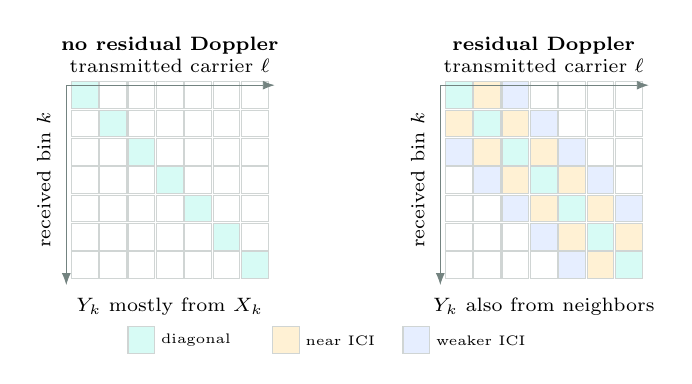
\begin{tikzpicture}[
  x=0.36cm,y=0.36cm,
  cell/.style={draw=labLine!22, minimum width=0.34cm, minimum height=0.34cm,
    inner sep=0pt},
  axis/.style={-{Latex[length=1.5mm]}, draw=labLine!65, line width=0.3pt},
  lbl/.style={font=\scriptsize, align=center},
  key/.style={font=\tiny, anchor=west}
]
\begin{scope}
  \node[lbl, font=\scriptsize\bfseries] at (3,1.75) {no residual Doppler};
  \foreach \i in {0,...,6} {
    \foreach \j in {0,...,6} {
      \node[cell, fill=white] at (\i,-\j) {};
    }
  }
  \foreach \i in {0,...,6} {
    \node[cell, fill=labTealLight] at (\i,-\i) {};
  }
  \draw[axis] (-0.65,0.35) -- (6.7,0.35);
  \draw[axis] (-0.65,0.35) -- (-0.65,-6.7);
  \node[lbl] at (3,1.05) {transmitted carrier $\ell$};
  \node[lbl, rotate=90] at (-1.45,-3) {received bin $k$};
  \node[lbl] at (3,-7.45) {$Y_k$ mostly from $X_k$};
\end{scope}

\begin{scope}[xshift=4.75cm]
  \node[lbl, font=\scriptsize\bfseries] at (3,1.75) {residual Doppler};
  \foreach \i in {0,...,6} {
    \foreach \j in {0,...,6} {
      \node[cell, fill=white] at (\i,-\j) {};
    }
  }
  \foreach \i/\j in {1/0,2/1,3/2,4/3,5/4,6/5,0/1,1/2,2/3,3/4,4/5,5/6} {
    \node[cell, fill=labGoldLight] at (\i,-\j) {};
  }
  \foreach \i/\j in {2/0,3/1,4/2,5/3,6/4,0/2,1/3,2/4,3/5,4/6} {
    \node[cell, fill=labBlueLight] at (\i,-\j) {};
  }
  \foreach \i in {0,...,6} {
    \node[cell, fill=labTealLight] at (\i,-\i) {};
  }
  \draw[axis] (-0.65,0.35) -- (6.7,0.35);
  \draw[axis] (-0.65,0.35) -- (-0.65,-6.7);
  \node[lbl] at (3,1.05) {transmitted carrier $\ell$};
  \node[lbl, rotate=90] at (-1.45,-3) {received bin $k$};
  \node[lbl] at (3,-7.45) {$Y_k$ also from neighbors};
\end{scope}
\node[cell, fill=labTealLight] at (2.0,-8.65) {};
\node[key] at (2.35,-8.65) {diagonal};
\node[cell, fill=labGoldLight] at (7.1,-8.65) {};
\node[key] at (7.45,-8.65) {near ICI};
\node[cell, fill=labBlueLight] at (11.7,-8.65) {};
\node[key] at (12.05,-8.65) {weaker ICI};
\end{tikzpicture}%
}
\caption{Origin of the ICI matrix. With an adequate CP and no residual Doppler,
the DFT diagonalizes the block channel, so each row of
$\mathbf H_{\mathrm{fd}}$ has energy mainly on its matching column. Residual
Doppler/time variation breaks that Fourier cancellation; row $k$ receives
energy from nearby columns, giving the off-diagonal ICI terms in
\eqref{eq:banded}.}
\label{fig:ici-origin-matrix}
\end{figure}

Let $\mathbf G$ be the post-acquisition, CP-removed linear operator over one
block. Then
$\mathbf Y=\mathbf F\mathbf G\mathbf F\Ht\mathbf X+\bm\nu\triangleq
\mathbf H_{\mathrm{fd}}\mathbf X+\bm\nu$, and if $\mathbf G$ is not circulant,
$\mathbf H_{\mathrm{fd}}$ is not diagonal:
\begin{equation}
  Y_k=H_{k,k}X_k+\!\!\sum_{\ell\in\mathcal B_K(k)\setminus\{k\}}\!\!H_{k,\ell}X_\ell
  +\epsilon_k^{(K)}+\nu_k,
  \label{eq:banded}
\end{equation}
with ICI neighborhood $\mathcal B_K(k)=\{\ell:\abs{\ell-k}\le K\}$. After
averaging over independent zero-mean coded data symbols, the truncation residual
has energy
$\E\abs{\epsilon_k^{(K)}}^2=\sum_{\ell\notin\mathcal B_K(k)}
\abs{H_{k,\ell}}^2\E\abs{X_\ell}^2$; deterministic pilots introduce cross-terms
unless averaged over pilot locations or payload realizations. For local residual
Doppler the off-diagonal energy concentrates near the main diagonal, so the
banded form is accurate at modest $K$. Equation~\eqref{eq:banded} is precisely
why a one-tap receiver
fails: it fits a diagonal model while the physical channel leaves a locally
coupled operator. The off-diagonal energy---the channel's \emph{dynamic
non-diagonality}---is the physical diagnostic motivating code-aware refinement,
although this paper does not estimate it as a per-capture predictor. In this
paper the banded form is a diagnostic model, not the
implemented estimator. Banded-ICI and sparse-channel receivers attempt to recover
the coupling coefficients $H_{k,\ell}$ or the path parameters that generate
them; the measured-channel \juna{} receiver instead observes partial-FFT
observation vectors and learns a local scalar combiner from pilots and decoder-derived soft
anchors.

The same notation also covers finite-CP stress. If the CP is shorter than the
effective delay spread, or if the channel varies across the useful interval, the
post-CP operator is not circulant. For OFDM symbol $s$ one can write
\begin{equation}
  \mathbf Y_s
  =\mathbf H_0\mathbf X_s
  +\mathbf J_{-}\mathbf X_{s-1}
  +\mathbf J_{+}\mathbf X_{s+1}
  +\bm\nu_s ,
  \label{eq:cp-short}
\end{equation}
where $\mathbf H_0$ is generally non-diagonal and $\mathbf J_{\pm}$ collect
inter-symbol leakage from neighboring OFDM symbols. Thus Doppler ICI and CP
shortfall both appear to the receiver as coupled-carrier/coupled-symbol
interference. \juna{} does not eliminate the need for a CP, but if this residual
coupling remains inside the partial-FFT combiner's effective model class, code
constraints can help the front end suppress it instead of relying only on pilots.

%=============================================================================
\section{Background: Partial-FFT Equalization}\label{sec:background}
\subsection{Partial-FFT Observation Vectors}
Partial-FFT reception retains information about intra-symbol time
variation~\cite{yerramalli2012partialfft}. With segment windows $g_p[n]$,
$p=1,\dots,N_{\rm view}$, the $p$-th observation for carrier $k$ is
$y_{p,k}=\tfrac{1}{\sqrt N}\sum_{n}g_p[n]r[n]e^{-j2\pi kn/N}$, stacked into
$\mathbf y_k\in\C^{N_{\rm view}}$. If the windows form a partition of unity then
$\sum_p y_{p,k}=Y_k$: the partial FFT invents no energy, it decomposes the full
FFT statistic into temporal views whose relative phases and amplitudes carry the
time-variation information.

\subsection{Pilot-Trained RLS Combiner}
The Partial~FFT+FEC baseline forms a scalar soft symbol with a bandwise linear
combiner $\widehat x_{k,s}=\mathbf w_{b}\Ht\mathbf y_{k,s}$, $k\in b$. In the
separate ReplayCh workbench used for the measured tables, one combiner per
frequency band is trained over the
current packet/candidate using pilot anchors $(k,s)\in\mathcal P_b$ against the
known $x_{k,s}$:
\begin{equation}
  \widehat{\mathbf w}_b=\arg\min_{\mathbf w}\!\!\sum_{(k,s)\in\mathcal P_b}\!\!
  \lambda^{\tau_{k,s}}\abs{x_{k,s}-\mathbf w\Ht\mathbf y_{k,s}}^2+\delta\norm{\mathbf w}_2^2,
  \label{eq:pfft-ls}
\end{equation}
with forgetting factor $\lambda$, sample age $\tau_{k,s}$ ($\tau=0$ for the most
recent RLS update), and ridge $\delta$. The recursion is initialized as
$\mathbf w_{b,0}=\mathbf 0$ and $\mathbf R_{b,0}=\delta^{-1}\mathbf I$, then
updated with gain $\mathbf g_i=\mathbf R_{i-1}\mathbf y_i/(\lambda+\mathbf
y_i\Ht\mathbf R_{i-1}\mathbf y_i)$, $\mathbf w_i=\mathbf w_{i-1}+\mathbf g_i
e_i^*$, and $\mathbf R_i=\lambda^{-1}(\mathbf R_{i-1}-\mathbf g_i\mathbf y_i\Ht
\mathbf R_{i-1})$. Partial~FFT+FEC is thus a strong baseline---time-window
diversity plus adaptive pilot-trained combining---but it remains a
pilot-only equalizer.

JunaCore evaluates the same pilot residual as a batch ridge-LS normal equation
with ridge $10^{-3}$ and 16 frequency bands. It first constructs the
Partial-FFT seed. If that candidate is invalid, it also evaluates the one-view
standard FFT candidate and uses it only when valid; this
\textbf{Standard-FFT fallback} prevents an invalid Partial-FFT seed from hiding a valid conventional
decode. All three public JunaCore profiles start from this shared rule.

%=============================================================================
\section{JUNA: A Coupled Objective}\label{sec:juna}
The pilot-trained combiner of Section~\ref{sec:background} fixes its weights from
pilots before decoding, so the LDPC code acts only after the soft symbols have
been formed. \juna{} removes that ordering at the level of the objective: it
replaces the pilot-stacked desired response with a packet-level forward model and
adds a differentiable parity penalty, so that pilots, partial-FFT observations, the
combiner, and the code constraints regularize one another within a single
problem. We state that ideal objective here; Section~\ref{sec:solver} describes
the bounded alternating procedure actually run on measured channels, which we do
not claim to be an exact minimizer of it.

\subsection{Packet Layout and Tanner-Graph Example}
\label{ssec:packet-tanner-example}
Fig.~\ref{fig:packet-tanner-example} shows the default JunaCore packet/Tanner
layout for $N=1024$, $N_{\rm cp}=256$, outer-pilot spacing three, inner-pilot
spacing two, and an LDPC $(n_b,k)=(1360,340)$ code. The left panel separates
the physical OFDM layer from the logical FEC layer. Outer pilots are
frequency-domain comb pilots on known subcarriers. Inner pilots are known
positions in the serialized message row before LDPC encoding; they are drawn as
violet anchors in the code stream, then transmitted on ordinary data tones after
encoding and modulation. The right panel shows an illustrative slice of the
sparse Tanner graph. JunaCore generates the parity-check matrix with the
Radford Neal LDPC tools using \texttt{evencol}, three check incidences per
codeword column, and the no-four-cycle option. Systematic encoding follows the
column permutation returned by \texttt{make-gen}; it does not assume an
identity parity suffix in the stored codeword order.

\begin{figure*}[t]
\centering
\scriptsize
\resizebox{0.98\textwidth}{!}{%
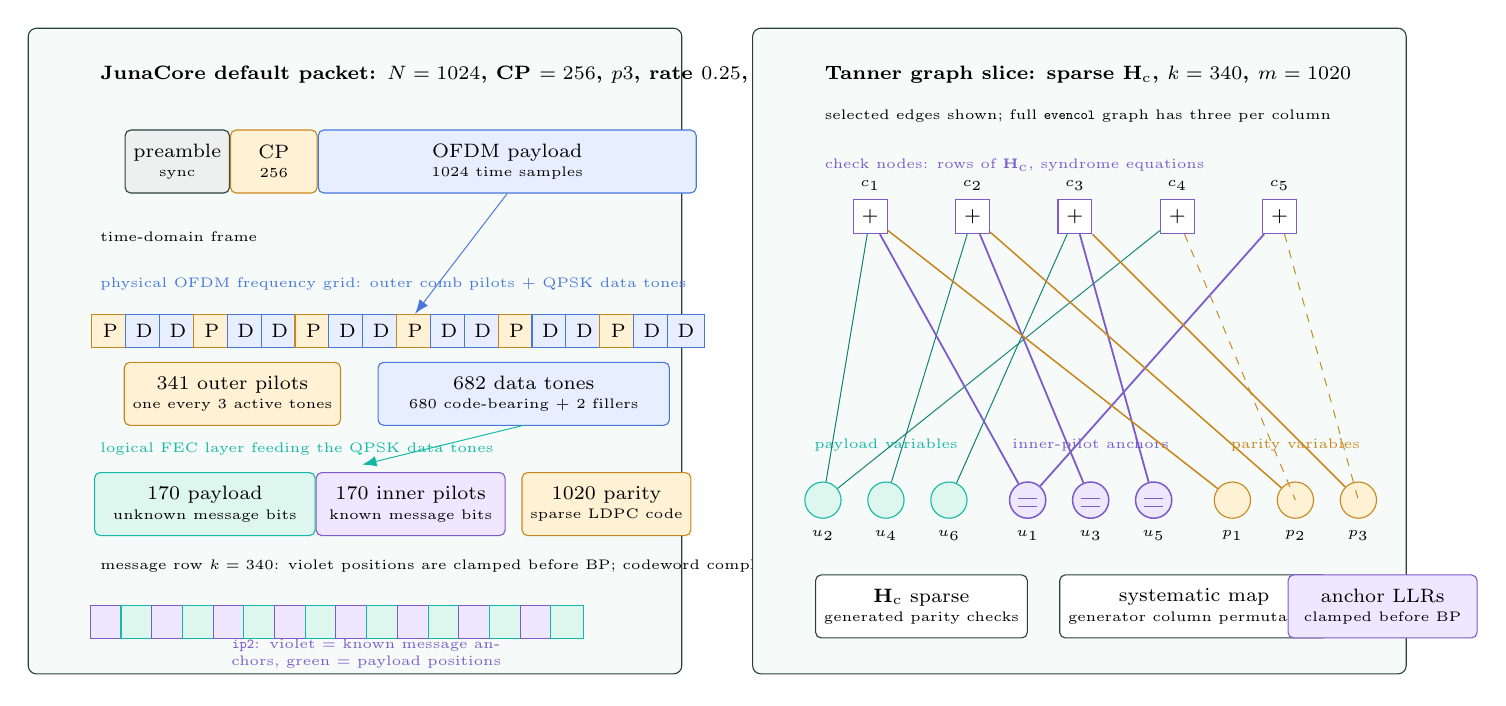
\begin{tikzpicture}[
  font=\scriptsize,
  tile/.style={draw, minimum width=4.7mm, minimum height=4.2mm, inner sep=0pt},
  box/.style={draw, rounded corners=2pt, align=center, inner sep=3pt,
    minimum height=8mm},
  title/.style={font=\scriptsize\bfseries, align=left},
  note/.style={font=\tiny, align=center},
  arr/.style={-{Latex[length=1.8mm]}, line width=0.35pt},
  edge/.style={line width=0.35pt},
  check/.style={draw=labViolet, fill=white, minimum size=4.3mm, inner sep=0pt},
  var/.style={circle, draw, minimum size=4.6mm, inner sep=0pt}
]
% --------------------------------------------------------------------------
% Left panel: packet structure, following the workbench packet canvas.
% --------------------------------------------------------------------------
\node[draw=labLine, fill=labPanel, rounded corners=3pt,
      minimum width=83mm, minimum height=82mm, anchor=north west] (packetPanel)
      at (0,0) {};
\node[title, anchor=west] at (0.8,-0.6)
  {JunaCore default packet: $N=1024$, CP $=256$, $p3$, rate $0.25$, $ip2$};

% Time-domain frame row.
\node[box, fill=labLine!8, draw=labLine, minimum width=13mm] (pre) at (1.9,-1.7)
  {preamble\\[-1pt]\tiny sync};
\node[box, fill=labGoldLight, draw=labGold, minimum width=11mm, right=0pt of pre] (cp)
  {CP\\[-1pt]\tiny 256};
\node[box, fill=labBlueLight, draw=labBlue, minimum width=48mm, right=0pt of cp] (payload)
  {OFDM payload\\[-1pt]\tiny 1024 time samples};
\node[note, anchor=west] at (0.8,-2.65) {time-domain frame};

% Frequency grid row.
\node[note, anchor=west, text=labBlue] at (0.8,-3.25)
  {physical OFDM frequency grid: outer comb pilots + QPSK data tones};
\foreach \i in {0,...,17} {
  \pgfmathtruncatemacro{\isp}{mod(\i,3)==0 ? 1 : 0}
  \ifnum\isp=1
    \node[tile, fill=labGoldLight, draw=labGold] (fg\i) at ({1.05+0.43*\i},-3.85) {P};
  \else
    \node[tile, fill=labBlueLight, draw=labBlue] (fg\i) at ({1.05+0.43*\i},-3.85) {D};
  \fi
}
\draw[arr, labBlue] (payload.south) -- (fg9.north);
\node[box, fill=labGoldLight, draw=labGold, minimum width=26mm] at (2.6,-4.65)
  {$341$ outer pilots\\[-1pt]\tiny one every 3 active tones};
\node[box, fill=labBlueLight, draw=labBlue, minimum width=37mm] at (6.3,-4.65)
  {$682$ data tones\\[-1pt]\tiny 680 code-bearing + 2 fillers};

% FEC layer row.
\draw[arr, labTeal] (6.3,-5.05) -- (4.25,-5.55);
\node[note, text=labTeal, anchor=west] at (0.8,-5.35)
  {logical FEC layer feeding the QPSK data tones};
\node[box, fill=labGreenLight, draw=labTeal, minimum width=28mm] (msgPay) at (2.25,-6.05)
  {$170$ payload\\[-1pt]\tiny unknown message bits};
\node[box, fill=labVioletLight, draw=labViolet, minimum width=24mm, right=0pt of msgPay] (msgAnc)
  {$170$ inner pilots\\[-1pt]\tiny known message bits};
\node[box, fill=labGoldLight, draw=labGold, minimum width=18mm, right=2mm of msgAnc] (parity)
  {$1020$ parity\\[-1pt]\tiny sparse LDPC code};
\node[note, anchor=west] at (0.8,-6.85)
  {message row $k=340$: violet positions are clamped before BP; codeword completes $n_b=1360$};

% Anchor placement row.
\foreach \i in {0,...,15} {
  \pgfmathtruncatemacro{\isa}{mod(\i,2)==0 ? 1 : 0}
  \ifnum\isa=1
    \node[tile, fill=labVioletLight, draw=labViolet, minimum width=4.1mm] at ({1.0+0.39*\i},-7.55) {};
  \else
    \node[tile, fill=labGreenLight, draw=labTeal, minimum width=4.1mm] at ({1.0+0.39*\i},-7.55) {};
  \fi
}
\node[note, text=labViolet, text width=56mm] at (4.3,-7.95)
  {\cfg{ip2}: violet = known message anchors, green = payload positions};

% --------------------------------------------------------------------------
% Right panel: Tanner graph slice, following the workbench Tanner canvas.
% --------------------------------------------------------------------------
\node[draw=labLine, fill=labPanel, rounded corners=3pt,
      minimum width=83mm, minimum height=82mm, anchor=north west] (tannerPanel)
      at (9.2,0) {};
\node[title, anchor=west] at (10.0,-0.6)
  {Tanner graph slice: sparse $\Hc$, $k=340$, $m=1020$};
\node[note, anchor=west] at (10.0,-1.12)
  {selected edges shown; full \texttt{evencol} graph has three per column};

% Check nodes.
\foreach \i/\x in {1/10.7,2/12.0,3/13.3,4/14.6,5/15.9} {
  \node[check] (c\i) at (\x,-2.4) {$+$};
  \node[note] at (\x,-2.0) {$c_{\i}$};
}
\node[note, anchor=west, text=labViolet] at (10.0,-1.75)
  {check nodes: rows of $\Hc$, syndrome equations};

% Variable nodes.
\foreach \name/\x/\lab in {u2/10.1/$u_2$,u4/10.9/$u_4$,u6/11.7/$u_6$} {
  \node[var, fill=labGreenLight, draw=labTeal] (\name) at (\x,-6.0) {};
  \node[note] at (\x,-6.45) {\lab};
}
\foreach \name/\x/\lab in {u1/12.7/$u_1$,u3/13.5/$u_3$,u5/14.3/$u_5$} {
  \node[var, fill=labVioletLight, draw=labViolet, line width=0.55pt] (\name) at (\x,-6.0) {};
  \draw[labViolet, line width=0.5pt] (\x-0.12,-5.98) -- (\x+0.12,-5.98);
  \draw[labViolet, line width=0.5pt] (\x-0.12,-6.08) -- (\x+0.12,-6.08);
  \node[note] at (\x,-6.45) {\lab};
}
\foreach \name/\x/\lab in {p1/15.3/$p_1$,p2/16.1/$p_2$,p3/16.9/$p_3$} {
  \node[var, fill=labGoldLight, draw=labGold] (\name) at (\x,-6.0) {};
  \node[note] at (\x,-6.45) {\lab};
}
\node[note, text=labTeal] at (10.9,-5.3) {payload variables};
\node[note, text=labViolet] at (13.5,-5.3) {inner-pilot anchors};
\node[note, text=labGold] at (16.1,-5.3) {parity variables};

% Selected edges from the generated sparse H_c.
\draw[edge, labTeal!70!black] (c1) -- (u2);
\draw[edge, labTeal!70!black] (c2) -- (u4);
\draw[edge, labTeal!70!black] (c3) -- (u6);
\draw[edge, labTeal!70!black] (c4) -- (u2);
\draw[edge, labViolet, line width=0.65pt] (c1) -- (u1);
\draw[edge, labViolet, line width=0.65pt] (c2) -- (u3);
\draw[edge, labViolet, line width=0.65pt] (c3) -- (u5);
\draw[edge, labViolet, line width=0.65pt] (c5) -- (u1);
\draw[edge, labGold, line width=0.55pt] (c1) -- (p1);
\draw[edge, labGold, line width=0.55pt] (c2) -- (p2);
\draw[edge, labGold, line width=0.55pt] (c3) -- (p3);
\draw[dashed, labGold, line width=0.35pt] (c4) -- (16.1,-6.0);
\draw[dashed, labGold, line width=0.35pt] (c5) -- (16.9,-6.0);

\node[box, fill=white, draw=labLine, minimum width=24mm, anchor=west] at (10.0,-7.35)
  {$\Hc$ sparse\\[-1pt]\tiny generated parity checks};
\node[box, fill=white, draw=labLine, minimum width=25mm, anchor=west] at (13.1,-7.35)
  {systematic map\\[-1pt]\tiny generator column permutation};
\node[box, fill=labVioletLight, draw=labViolet, minimum width=24mm, anchor=west] at (16.0,-7.35)
  {anchor LLRs\\[-1pt]\tiny clamped before BP};
\end{tikzpicture}%
}
\caption{JunaCore default packet-structure and Tanner-graph example. The
physical OFDM layer has 1023 active tones per symbol (only DC is excluded),
split into 341 outer frequency-domain pilots and 682 data tones. The logical
FEC layer maps $k=340$ message bits and 1020 parity bits to $n_b=1360$ coded
bits. The codeword occupies 680 QPSK data tones; the remaining
two deterministic filler tones complete the OFDM data grid. Inner pilots are
known positions inside the message row ($170$ anchors for \cfg{ip2}); they are
not extra OFDM pilot tones. In the Tanner graph, violet anchor variables enter
BP with clamped LLRs, green payload variables are unknown, and gold parity
variables participate in the same generated sparse matrix. The systematic
generator may permute codeword columns, while every encoded vector still
satisfies $\Hc\mathbf b\T=\mathbf0$.}
\label{fig:packet-tanner-example}
\end{figure*}

\subsection{Bit Latents, Soft QPSK Symbols, and a Parity Surrogate}
\label{ssec:ldpc}
An LDPC code is fixed by a sparse parity-check matrix $\Hc\in\F_2^{m\times
n_b}$ with $n_b$ coded bits and $m$ checks~\cite{gallager1963ldpc}; an encoder
maps $\mathbf u$ to a codeword $\mathbf b$ with $\Hc\mathbf b\T=\mathbf 0$
over $\F_2$. Belief propagation (BP) on the induced Tanner graph remains the
hard-decision decoder~\cite{richardson2008modern}. The JunaCore implementation
invokes the Radford Neal \texttt{make-ldpc} and \texttt{make-gen} tools. Its
default $(1360,340)$ code uses \texttt{evencol} with three incidences per
codeword column and a fixed seed, then stores the systematic generator
permutation returned by \texttt{make-gen}. Thus $k$ message bits are mapped to
$n_b$ coded bits with rate $k/n_b$, but the sparse parity-check matrix is not
required to have the raw form $[\Hm\ \mathbf I]$ in codeword order. Some message
positions can be fixed as \emph{inner pilots}; these are known bits inside the
LDPC message, distinct from outer OFDM pilot tones, and their LLRs are clamped
during BP. The payload BER and PSR reported below exclude these inner-pilot
message positions. Thus the LDPC design rate is $k/n_b$, while the net unknown
payload rate is lower when inner-pilot message positions are reserved as known
anchors.

For message vector $\mathbf u$, encoding solves for a systematic codeword in the
generator's permuted column order and verifies $\Hc\mathbf b\T=\mathbf0$ over
$\F_2$. The fixed seed makes this code deterministic, and all package receiver
profiles share the same cached code instance. This is a reproducible sparse
LDPC construction, not a claim that the generated graph is an optimized
acoustic code.

Because the code constraints are binary while the subcarriers carry QPSK, the bit
and symbol variables are kept separate. Let $\xi_i=\tanh(z_i/2)\in(-1,1)$ be the
relaxed bipolar variable for coded bit $b_i$, so hard bits satisfy
$\xi_i=1-2b_i$. For Gray-labeled QPSK, data carrier $k$ carries bits
$i_1(k),i_2(k)$ and its relaxed symbol is
\begin{equation}
  s_k(\mathbf z)=\tfrac{1}{\sqrt2}\big(\xi_{i_1(k)}(\mathbf z)
  +j\,\xi_{i_2(k)}(\mathbf z)\big),
  \label{eq:qpsk-soft}
\end{equation}
while pilots use known $s_p=P_p$. With check neighborhoods $\{\mathcal N_j\}$,
the differentiable parity surrogate is
\begin{equation}
  \mathcal R_{\mathrm{par}}(\mathbf z)
  =\sum_{j=1}^{m}\Big(1-\prod_{i\in\mathcal N_j}\xi_i(\mathbf z)\Big)^2 ,
  \label{eq:soft-parity}
\end{equation}
which equals $0$ exactly when every check is satisfied for hard bipolar bits, so
$\mathcal R_{\mathrm{par}}$ is a smooth code regularizer that preserves the
binary/complex distinction.
This surrogate is used as a differentiable consistency penalty in the objective
lens and gradient diagnostics; the implemented receiver relies on BP for the
actual code update because direct optimization of high-degree parity products
can be poorly conditioned and can have weak gradients.

This parity structure is the mathematical reason code information can provide
training equations beyond the physical pilots. With pilots alone, the combiner in
band $b$ is identified only from $\mathcal P_b$. After BP, a data carrier with
posterior mean $\widetilde x_{d,s}=\mathbb E[X_{d,s}\mid\mathbf Y]$ and
confidence $c_{d,s}$ can contribute an additional soft equation. A weighted batch
view of the update is
\begin{equation}
  \begin{aligned}
  \widehat{\mathbf w}_b
  =\arg\min_{\mathbf w}\;&
  \sum_{(p,s)\in\mathcal P_b}
      \abs{P_{p,s}-\mathbf w\Ht\mathbf y_{p,s}}^2\\
  &+\sum_{(d,s)\in\mathcal D_b^+}c_{d,s}
      \abs{\widetilde x_{d,s}-\mathbf w\Ht\mathbf y_{d,s}}^2\\
  &+\delta\norm{\mathbf w}_2^2 ,
  \end{aligned}
  \label{eq:soft-pilot-ls}
\end{equation}
where $\mathcal D_b^+$ is the selected data-anchor set and $c_{d,s}$ is its
posterior-confidence weight. The JunaCore reference implementation gives every
physical pilot unit weight and every selected data target its confidence, then
solves this batch ridge-LS problem with $\delta=10^{-3}$. Its default threshold
is zero, its data-anchor cap is unbounded, and it performs at most two refinement
passes with early exit on a valid or non-improving candidate. Compared with the
pilot-only solve, the normal matrix gains data-anchor terms
$\sum_{(d,s)\in\mathcal D_b^+}c_{d,s}\mathbf y_{d,s}\mathbf y_{d,s}\Ht$.
When the decoder posterior is informative, those terms improve conditioning just
as additional pilots would; when it is uninformative or biased, retained physical
pilots, posterior means rather than hard slices, optional confidence
thresholding/caps, and candidate selection limit the damage. The separate
ReplayCh workbench uses recursive RLS updates and a finite benchmark anchor cap;
those measured-run settings must not be read as JunaCore package defaults.

\subsection{The Coupled Objective}\label{ssec:juna-objective}
Let $\mathbf Y_k\in\C^M$ collect the $M$ partial-FFT observations at
carrier $k$, $\mathbf w_k$ the combiner forming $\widehat s_k=\mathbf
w_k\Ht\mathbf Y_k$, and $\mathbf c_{k,q}\in\C^M$ the partial-FFT-domain response from carrier
$q$ to $k$. With banded support $\mathcal B_K(k)$, the forward model is $\mathbf
Y_k=\sum_{q\in\mathcal B_K(k)}\mathbf c_{k,q}s_q(\mathbf z)+\mathbf n_k$, and
the ideal joint surrogate is
\begin{equation}
  \begin{aligned}
    \mathcal L(\mathbf C,\mathbf W,\mathbf z)
    ={}&\lambda_{\mathrm d}\sum_{k\in\mathcal K}
        \Big\|\mathbf Y_k-\sum_{q\in\mathcal B_K(k)}
        \mathbf c_{k,q}s_q(\mathbf z)\Big\|_{\Sigma_k^{-1}}^2\\
    &+\eta\sum_{p\in\mathcal P}\abs{\mathbf w_p\Ht\mathbf Y_p-P_p}^2\\
    &+\rho\sum_{k\in\mathcal D}
      \abs{\mathbf w_k\Ht\mathbf Y_k-s_k(\mathbf z)}^2\\
    &+\gamma_C\norm{\mathbf C}_F^2+\gamma_W\sum_{k}\norm{\mathbf w_k}_2^2\\
    &+\gamma_S\sum_{k}\norm{\mathbf w_{k+1}-\mathbf w_k}_2^2
      +\lambda_{\mathrm p}\,\mathcal R_{\mathrm{par}}(\mathbf z).
  \end{aligned}
  \label{eq:juna-total}
\end{equation}
The first term enforces observation consistency; the second anchors pilots; the
third ties combiner outputs to the relaxed data symbols; the rest regularize
partial-FFT-domain model size, combiner energy, frequency smoothness, and parity.
$\Sigma_k=\sigma^2\mathbf I$ recovers ordinary squared error. This objective is
not intended as an identifiable physical channel estimator: the partial-FFT-domain response
tensor $\mathbf C$ and combiner $\mathbf W$ are coupled through the symbols,
pilots, and regularizers, but no explicit constraint forces $\mathbf W$ to be the
inverse of $\mathbf C$. Its role is to show how observation-vector consistency, combiner
outputs, pilots, and code constraints can be placed in one regularized problem.
Multiple $(\mathbf C,\mathbf W,\mathbf z)$ triples can explain the same partial-FFT
observations; $\mathbf C$ is included to expose the coupled-carrier structure,
not to claim unique identification of the physical ICI matrix.

The deployed \junawcz{} receiver of Section~\ref{ssec:juna-wcz} resolves this
underdetermination structurally rather than by regularization alone. With $M$
partial-FFT views, each carrier contributes $M$ complex observation equations,
while an unconstrained per-carrier response column introduces $M(2K{+}1)$
unknowns; the observation term can therefore be driven to zero for \emph{any}
latent vector $\mathbf z$ once $\gamma_C=0$, and contributes no information
about the transmitted bits. Tying $\mathbf c_{k,q}$ across the same $B$
frequency bands that already tie the combiner restores an overdetermined
per-band fit whenever a band holds more than $2K{+}1$ carriers, which makes
observation consistency informative about $\mathbf z$ while preserving the
coupled structure of~\eqref{eq:juna-total}.

Equation~\eqref{eq:juna-total} is written for a single-symbol carrier
neighborhood. Under CP-short leakage, the index can be lifted from $k$ to
$(k,s)$ and $\mathcal B_K(k)$ replaced by a local space-time neighborhood that
also contains neighboring OFDM symbols:
\begin{equation}
  \mathbf Y_{k,s}
  =\sum_{(q,r)\in\mathcal B(k,s)}
      \mathbf c_{k,s;q,r}\,s_{q,r}(\mathbf z)+\mathbf n_{k,s}.
  \label{eq:space-time-coupling}
\end{equation}
The same pilot, data-anchor, smoothness, and parity terms then regularize
whether the coupling came from Doppler ICI, insufficient CP, or both. This is a
modeling extension, not a CP-short experiment in this paper: it shows how code
structure could add global parity constraints to an otherwise underconstrained
front-end fit, but the measured results below should not be read as a validated
CP-relaxation rule.

\subsection{Relation to the Pilot-Trained Combiner}\label{ssec:juna-relation}
\juna{} is the natural lifting of~\eqref{eq:pfft-ls}: the pilot-only desired
response is replaced by the packet-level partial-FFT-domain model, every carrier refines the
front end, the data field is generated by bit latents so soft bits improve during
inference, and the code enters through~\eqref{eq:soft-parity}. Equation
\eqref{eq:juna-total} is best read as a theoretical lens---it is not the exact
algorithm run on measured channels. Of the deployed receivers, \junalite{} and
\junawz{} do not estimate $\mathbf C$; the constrained \junawcz{} receiver of
Section~\ref{ssec:juna-wcz} estimates a band-tied, $K{=}1$ counterpart of it
jointly with $(\mathbf W,\mathbf z)$, while the full per-carrier tensor remains
a theoretical lens that makes explicit the physical coupling motivating every
update below.
The operative connection is narrower: \junawz{} freezes the partial-FFT-domain model and
descends a reduced $(\mathbf W,\mathbf z)$ objective, while \junalite{} uses the
fixed-$\mathbf z$ view to turn the tie term into an RLS target-fitting problem
for the combiner. With the combiner fixed, BP supplies the parity-aware
posterior used for the next latent-symbol or anchor update.
Section~\ref{sec:solver} makes this alternation, and its limits, precise.

%=============================================================================
\section{Implemented Receivers: \texorpdfstring{\junawz{}}{JUNA-Wz},
\texorpdfstring{\junalite{}}{JUNA-lite}, and
\texorpdfstring{\junawcz{}}{JUNA-WCz}}\label{sec:solver}
We implement three receivers derived from the coupled objective. The
reduced gradient receiver, \junawz{}, freezes the explicit partial-FFT-domain response
tensor $\mathbf C$ at the partial-FFT observation model and updates the
partial-FFT combiner $\mathbf W$ together with the soft bit latents $\mathbf z$.
Its coordinates are weighted by decoder confidence, and each refined state is
decoded and compared as a candidate (Section~\ref{ssec:gradient-juna}); BP
projection is not applied inside Adam.
Because that solve repeats gradient steps and decodes per packet, we also
implement \junalite{}, a lightweight approximation that replaces explicit
gradient descent with a bounded posterior-anchor batch ridge-LS refit
(Section~\ref{ssec:junalite}). It keeps the same partial-FFT observation model
and combiner but re-estimates the combiner \emph{toward} decoder posterior means.
\junalite{} costs at most two ridge-LS/BP refinement passes per packet. The
related ReplayCh Lite profile carries the large-scale measured sweeps, while
\junawz{} is the gradient mirror used to check the approximation. Both receivers
share the LDPC decode pass and the decoder-grounded candidate selection
described next, and differ only in how the combiner and data symbols move
between decodes. The full $(\mathbf W,\mathbf C,\mathbf z)$ optimizer,
\junawcz{}, is a public package profile with controlled diagnostic evidence,
but it is not part of the measured replay sweeps.
Fig.~\ref{fig:juna-iterative-loop} gives the receiver loop as a pictorial
summary: the top row is the seed Partial-FFT/FEC path, and the dashed paths are
the decoder-to-front-end feedback used by \junalite{} and \junawz{}.
Algorithms~\ref{alg:junalite} and~\ref{alg:junawz} list the two deployed
updates in the same notation.

\subsection{External ReplayCh workbench algorithms: OFDM5 Prototype Solvers}
\label{ssec:ofdm5-prototypes}
For clarity, we also record optimization paths from the external ReplayCh
workbench. These OFDM5, SPADE, and ForwardDiff paths are useful implementation
lineage, but they are not modules under JunaCore's \texttt{src/} tree and do not
define the package behavior tested in this repository. OFDM5 contains
three inner mechanisms: a block-coordinate least-squares solver for a local ICI
combiner, a manually differentiated code-aware partial-FFT solver, and optional
ForwardDiff-based symbol refiners. A decoder-aware wrapper around the
block-coordinate solver is also summarized below, because that wrapper is the
code path that supplies the pseudo-pilot vector used by the second
block-coordinate pass.

Let \(V\) be the number of partial-FFT temporal views and define
\(\mathbf y_k=[Y_{1,k},\ldots,Y_{V,k}]^T\). The local ICI solver divides the
FFT bins into \(B\) frequency bands,
\begin{equation}
  b(k)=1+\left\lfloor \frac{(k-1)B}{N}\right\rfloor,
  \qquad b(k)\in\{1,\ldots,B\},
  \label{eq:ofdm5-band-index}
\end{equation}
and first builds the ``safe'' pilot-neighborhood bins
\begin{equation}
  \Omega_K=\{k:\; k-\Delta \in \mathcal P
      \;\text{for all}\; \Delta=-K,\ldots,K\},
  \label{eq:ofdm5-safe-pilots}
\end{equation}
where indexing is circular modulo \(N\). In the ordinary pilot-only mode the
training set is \(\Omega_{\rm tr}=\Omega_K\), \(s_k^{\rm ref}=s_{\rm pilot}\),
and \(\rho_k=1\). When \texttt{pseudo\_enable} is true and a fixed symbol vector
\(\mathbf s^{\rm fixed}\) is supplied, OFDM5 replaces the safe-pilot set by
weighted pilot-plus-decision training,
\begin{equation}
\begin{aligned}
  \kappa_k&=\operatorname{clip}
      \left(\abs{s_k^{\rm fixed}}/\abs{s_{\rm pilot}},0,1\right),\\
  \nu_k&=\rho_{\rm data}\kappa_k^{p_{\rm conf}},\\
  s_k^{\rm ref} &=
  \begin{cases}
    s_{\rm pilot}, & k\in\mathcal P,\\
    s_k^{\rm fixed}, & k\notin\mathcal P,
  \end{cases}\\
  \rho_k &=
  \begin{cases}
    1, & k\in\mathcal P,\\
    \nu_k, & k\notin\mathcal P,\ \nu_k\ge\rho_{\min},\\
    0, & \text{otherwise},
  \end{cases}\\
  \Omega_{\rm tr}&=\{k:\rho_k>0\}.
\end{aligned}
  \label{eq:ofdm5-pseudo-training}
\end{equation}
Thus pseudo-training uses the decided symbol on a data tone itself, rather than
requiring every neighboring tone to be a true pilot. For band \(b\), the combiner is
\(\mathbf w_b\in\C^V\), the local ICI coefficients are
\(\mathbf c_b=[C_{-K,b},\ldots,C_{K,b}]^T\), and the pilot or pseudo-pilot
reference on tone \(q\) is \(s_q^{\rm ref}\). With optional nonnegative training
weights \(\rho_k\), the OFDM5 weighted objective is
\begin{equation}
\begin{aligned}
  a_{k,\Delta}&=H_{k-\Delta}s_{k-\Delta}^{\rm ref},\\
  e_k
  ={}&\mathbf w_{b(k)}^H\mathbf y_k
      -\sum_{\Delta=-K}^{K}
        C_{\Delta,b(k)}a_{k,\Delta},\\
  J_{\rm WC}(\mathbf W,\mathbf C)
  ={}&\sum_{k\in\Omega_{\rm tr}}\rho_k\abs{e_k}^2\\
  &+\eta_W\sum_b\norm{\mathbf w_b}_2^2\\
  &+\eta_C\sum_b\norm{\mathbf c_b}_2^2\\
  &+\gamma_C\sum_b\norm{\mathbf D\mathbf c_b}_2^2 ,
\end{aligned}
  \label{eq:ofdm5-wc-loss}
\end{equation}
where \(\mathbf D\) is the first-difference matrix. The default OFDM5
\texttt{:wc} path does not differentiate this loss. It alternates two normal
equation solves. Holding \(\mathbf C\) fixed, form one row per training tone in
band \(b\),
\begin{equation}
  (\mathbf Y_b)_{k,:}=\sqrt{\rho_k}\,\mathbf y_k^T,\qquad
  t_{b,k}=\sqrt{\rho_k}\sum_{\Delta=-K}^{K}
      C_{\Delta,b}H_{k-\Delta}s_{k-\Delta}^{\rm ref}.
  \label{eq:ofdm5-w-matrix}
\end{equation}
The code solves for \(\mathbf u_b=\overline{\mathbf w_b}\),
\begin{equation}
  \mathbf u_b
  =(\mathbf Y_b^H\mathbf Y_b+\eta_W\mathbf I)^{-1}\mathbf Y_b^H\mathbf t_b,
  \qquad
  \mathbf w_b=\overline{\mathbf u_b}.
  \label{eq:ofdm5-w-step}
\end{equation}
Holding \(\mathbf W\) fixed, form
\begin{equation}
  (\mathbf A_b)_{k,\Delta}
  =\sqrt{\rho_k}\,H_{k-\Delta}s_{k-\Delta}^{\rm ref},\qquad
  r_{b,k}=\sqrt{\rho_k}\,\mathbf w_b^H\mathbf y_k .
  \label{eq:ofdm5-c-matrix}
\end{equation}
Then
\begin{equation}
  \mathbf c_b
  =\left(\mathbf A_b^H\mathbf A_b
      +\eta_C\operatorname{diag}(\mathbf q_b)
      +\gamma_C\mathbf D^T\mathbf D\right)^{-1}
    \mathbf A_b^H\mathbf r_b ,
  \label{eq:ofdm5-c-step}
\end{equation}
where \(\mathbf q_b=\mathbf 1\) unless the sparse-support prior is active
(\texttt{c\_sparse\_enable}, positive \texttt{c\_sparse\_topk}, positive
\texttt{c\_sparse\_offdiag\_boost}, and \(2K+1>1\)). In that case the code
scores the columns by
\(\abs{\mathbf A_b^H\mathbf r_b}\), always keeps the center delay, keeps the
largest \texttt{c\_sparse\_topk} scores, and adds
\texttt{c\_sparse\_offdiag\_boost} to the other diagonal penalties. Empty bands
retain the previous estimate; without a previous estimate, the \(\mathbf W\)
fallback is the uniform combiner \((1,\ldots,1)^T/\sqrt V\) and the
\(\mathbf C\) fallback is the center-tap identity. After each solve, OFDM5
optionally normalizes
\(\mathbf w_b\leftarrow\mathbf w_b/(\norm{\mathbf w_b}_2+\epsilon)\) and
rotates/scales \(\mathbf c_b\) by dividing by
\(\abs{C_{0,b}}+\epsilon\) and multiplying by \(e^{-j\angle C_{0,b}}\), so that
the center coefficient is real and close to one. If a direct spectrum
\(\mathbf x^{\rm fixed}\) is supplied, the code blends
\begin{equation}
  \mathbf x
  =\alpha\,\mathbf x_{\rm model}+(1-\alpha)\mathbf x^{\rm fixed},
  \qquad
  \alpha=\operatorname{clip}(\texttt{xblend},0,1),
  \label{eq:ofdm5-xblend}
\end{equation}
and if \texttt{use\_w=false}, \(\mathbf x^{\rm fixed}\) is required and the
\(\mathbf W\)-step is skipped. The demixing stage then approximately inverts the
local ICI operator \(\mathcal C\) by guarded Richardson iteration,
\begin{equation}
  \mathbf z^{(r+1)}
  =\mathbf z^{(r)}+\mu\big(\mathbf x-\mathcal C\mathbf z^{(r)}\big),
  \qquad
  \mathbf x_k=\mathbf w_{b(k)}^H\mathbf y_k ,
  \label{eq:ofdm5-richardson}
\end{equation}
with \(\mu=\texttt{demix\_safety}/\widehat{\norm{\mathcal C}}\) chosen from a
power-iteration norm estimate when \(\mu\) is not supplied. The guard stores the
previous iterate; if a step gives a nonfinite residual or exceeds
\texttt{demix\_guard\_factor} times the initial residual, the code rolls back to
the previous iterate and terminates. It also stops early once the residual falls
below \(10^{-6}\) of its initial value.

\begin{algorithm}[t]
\caption{OFDM5 block-coordinate LS local-ICI solver}
\label{alg:ofdm5-wc}
\footnotesize
\begin{algorithmic}[1]
\Require Partial-FFT views \(\mathbf y_k\), pilot mask, channel estimate
  \(H_k\), optional fixed symbols \(\mathbf s^{\rm fixed}\), optional direct
  spectrum \(\mathbf x^{\rm fixed}\), half-bandwidth \(K\), bands \(B\),
  iterations \(T\)
\State Build \(\Omega_{\rm tr}\): use~\eqref{eq:ofdm5-safe-pilots} in pilot-only
  mode, or~\eqref{eq:ofdm5-pseudo-training} in pseudo-training mode.
\State Initialize \(\mathbf w_b=(1,\ldots,1)^T/\sqrt V\) and
  \(C_{0,b}=1,\;C_{\Delta\ne0,b}=0\).
\For{\(t=1,\ldots,T\)}
  \If{\texttt{use\_w} and \(\mathbf W\) is not frozen}
    \For{each band \(b\)}
      \State Build \(\mathbf Y_b,\mathbf t_b\) from~\eqref{eq:ofdm5-w-matrix}.
      \State Solve~\eqref{eq:ofdm5-w-step}; optionally normalize \(\mathbf w_b\).
    \EndFor
  \EndIf
  \If{\(\mathbf C\) is not frozen}
    \For{each band \(b\)}
      \State Build \(\mathbf A_b,\mathbf r_b\) from~\eqref{eq:ofdm5-c-matrix};
        if \texttt{use\_w=false}, replace \(r_{b,k}\) by
        \(\sqrt{\rho_k}x^{\rm fixed}_k\).
      \State Solve~\eqref{eq:ofdm5-c-step}; optionally normalize \(\mathbf c_b\).
    \EndFor
  \EndIf
  \State Record \(J_{\rm WC}\) from~\eqref{eq:ofdm5-wc-loss}.
\EndFor
\State Compute \(x_{{\rm model},k}=\mathbf w_{b(k)}^H\mathbf y_k\), or
  use \(\mathbf x^{\rm fixed}\) when \texttt{use\_w=false}.
\State If \(\mathbf x^{\rm fixed}\) is present, blend by~\eqref{eq:ofdm5-xblend}.
\If{demixing is enabled}
  \State Run~\eqref{eq:ofdm5-richardson} to obtain \(\mathbf z\).
\Else
  \State Set \(\mathbf z=\mathbf x\).
\EndIf
\State Optionally call the AD symbol refiner in Algorithm~\ref{alg:ofdm5-ad}.
\State \Return \(\mathbf W,\mathbf C,\mathbf x,\mathbf z\).
\end{algorithmic}
\end{algorithm}

The decoder-aware OFDM5 wrapper uses Algorithm~\ref{alg:ofdm5-wc} as an inner
solver. It first runs a seed block-coordinate pass, forms data-bin LLRs from the
demixed symbols after optional one-tap equalization,
\(\tilde s_i=H_i^*z_i/(\abs{H_i}^2+\epsilon)\), and calls BP with half-LLR
messages. For QPSK pseudo-training, the BP bit probabilities are converted into
soft constellation points
\begin{equation}
  s^{\rm BP}_{d_i}
  =\frac{1}{\sqrt2}\left[
    \operatorname{clip}(1-2p_{2i-1})+
    j\,\operatorname{clip}(1-2p_{2i})\right],
  \label{eq:ofdm5-wrapper-soft-qpsk}
\end{equation}
while pilot tones are reset to \(s_{\rm pilot}\). The wrapper then builds
\(\mathbf s^{\rm fixed}=\mathbf s^{\rm BP}\),
\(\mathbf x^{\rm fixed}=H_{\rm raw}\odot\mathbf s^{\rm fixed}\), and reruns the
block-coordinate solver warm-started from the first pass's \(\mathbf W,\mathbf C\)
with pseudo-training enabled. It keeps the better decode by validity first,
then syndrome weight, optionally mean \(|{\rm LLR}|\), and finally BP iteration
count. If the optional LLR-domain refinement is enabled, OFDM5 optimizes
\begin{equation}
\begin{aligned}
  \eta_m(\boldsymbol\ell)
  &=1-\prod_{r\in\mathcal N(m)}
    \operatorname{clip}\!\left(\tanh(\ell_r/2)\right),\\
  J_{\ell}(\boldsymbol\ell)
  ={}&\sigma^{-2}\norm{
    \mathcal S_\epsilon\operatorname{diag}(H)\mathbf X(\boldsymbol\ell)
    -\mathbf z}_2^2\\
  &+\lambda\sum_m\eta_m(\boldsymbol\ell)^2
    +\gamma\norm{\boldsymbol\ell}_2^2 ,
\end{aligned}
  \label{eq:ofdm5-wrapper-llr-loss}
\end{equation}
where \(\mathcal S_\epsilon=\mathbf F\operatorname{diag}
(e^{j2\pi\epsilon n/N})\mathbf F^H\) is applied by FFTs and
\(\mathbf X(\boldsymbol\ell)\) is the QPSK soft-symbol map using
\(\tanh(\ell/2)\). This branch uses manual gradients inside an L-BFGS optimizer,
then applies the same BP and decode-preference policy.

The same OFDM5 entry point also has a separate \texttt{:wh} mode. This branch
requires \texttt{use\_w=true} and does not estimate the local ICI matrix
\(\mathbf C\). Instead it alternates the banded combiner with a length-\(L\)
channel impulse response \(\mathbf h\), with
\(H(\mathbf h)=\operatorname{FFT}([\mathbf h;0])\):
\begin{equation}
\begin{aligned}
  J_{\rm WH}(\mathbf W,\mathbf h)
  ={}&\sum_{k\in\mathcal P}
    \abs{\mathbf w_{b(k)}^H\mathbf y_k-H_k(\mathbf h)s_{\rm pilot}}^2\\
  &+\eta_W\norm{\mathbf W}_F^2
    +\mathbf h^H\boldsymbol\Lambda_{\rm wh}\mathbf h
    +\mu_{\rm wh}\norm{\mathbf h}_1 .
\end{aligned}
  \label{eq:ofdm5-wh-loss}
\end{equation}
The delay taper used here and in SPADE is
\begin{equation}
\begin{aligned}
  [\boldsymbol\Lambda]_{\ell,\ell}
  &=\lambda_0\left(1+\frac{\ell}{L_\star}\right)^2,\\
  L_\star&=
  \begin{cases}
    L_{\rm decay}, & L_{\rm decay}>0,\\
    \max(L/4,1), & L_{\rm decay}\le0,
  \end{cases}
\end{aligned}
  \label{eq:ofdm5-delay-taper}
\end{equation}
for tap index \(\ell=0,\ldots,L-1\); SPADE's ISTA weights use the same taper
with \(\lambda_0=1\). In \texttt{:wh} mode the \texttt{freeze\_c} flag freezes
this \(\mathbf h\)-step.
The implementation initializes \(\mathbf h\) by fitting \(H_{\rm raw}\) over all
tones with a tapered ridge penalty, solves \(\mathbf W\) on all pilot tones using
targets \(H_k(\mathbf h)s_{\rm pilot}\), then re-estimates \(\mathbf h\) from
\begin{equation}
  z^{\rm pilot}_k
  =(1-\rho_{\rm anchor})
    \frac{\mathbf w_{b(k)}^H\mathbf y_k}{s_{\rm pilot}}
    +\rho_{\rm anchor}H_{{\rm raw},k},\qquad k\in\mathcal P .
\label{eq:ofdm5-wh-zpilot}
\end{equation}
The \(\mathbf h\)-step is a tapered LS fit of
\(\mathbf F_{\mathcal P,L}\mathbf h\approx \mathbf z^{\rm pilot}\), with optional
complex soft-thresholding. The returned \(\mathbf C\) field is only a zero
placeholder in this mode; downstream code uses \(H(\mathbf h)\) and the same
\(\mathbf x^{\rm fixed}\) blend and optional BPSK code refiner as above, but it
does not run the Richardson demixing stage.

OFDM5 also contains a manually differentiated solver, named SPADE in that
codebase, that fits a longer channel and QPSK soft symbols directly to the
partial-FFT observation matrix. The code requires \(V\) to divide \(N\) and works
with the unitary observation
\begin{equation}
\begin{aligned}
  \mathbf Y_u&=\frac{\mathbf Y_p}{\texttt{scaleYp}\sqrt N},\\
  \texttt{scaleYp}&=
  \begin{cases}
    \sqrt V, & V>1,\\
    1, & V=1.
  \end{cases}
\end{aligned}
  \label{eq:ofdm5-spade-yu}
\end{equation}
Let \(\mathcal A_H(\mathbf X)\) denote the
matrix-free operator that maps a frequency-domain symbol vector \(\mathbf X\)
through frequency response \(H\), a unitary IFFT, temporal windowing into
\(V\) partial-FFT views, and unitary FFTs back to the observation grid. For data
tone \(d_i\), OFDM5 parameterizes the QPSK soft symbol by logits
\begin{equation}
\begin{aligned}
  s^R_i&=\operatorname{clip}(\tanh u_{2i-1},-c_{\rm soft},c_{\rm soft}),\\
  s^I_i&=\operatorname{clip}(\tanh u_{2i},-c_{\rm soft},c_{\rm soft}),\\
  X_{d_i}(\mathbf u)
  &=\frac{1}{\sqrt2}\big(s^R_i+js^I_i\big).
\end{aligned}
  \label{eq:ofdm5-spade-soft-symbol}
\end{equation}
while pilot tones remain fixed. For fixed \(H\), the symbol-step loss is
\begin{equation}
\begin{aligned}
  J_u(\mathbf u;H)
  ={}&\sigma^{-2}\norm{\mathcal A_H(\mathbf X(\mathbf u))-\mathbf Y_u}_F^2\\
  &+\lambda_{\rm anchor}\sum_i
      \abs{X_{d_i}(\mathbf u)-X_{{\rm anchor},d_i}}^2\\
  &+\lambda_{\rm code}\sum_{m}
      \left(1-\prod_{\ell\in\mathcal N(m)}
      \operatorname{clip}(\tanh u_\ell)\right)^2\\
  &+\lambda_{\rm hard}\sum_\ell \left(1-s_\ell^2\right),
\end{aligned}
  \label{eq:ofdm5-spade-u-loss}
\end{equation}
The implementation computes the residual
\(\mathbf R=\mathcal A_H(\mathbf X(\mathbf u))-\mathbf Y_u\), applies the
adjoint partial-FFT operator to obtain
\begin{equation}
  \mathbf g_X
  =2\sigma^{-2}\mathcal A_H^*(\mathbf R),
  \label{eq:ofdm5-spade-adjoint}
\end{equation}
and then chains through \(X_{d_i}(\mathbf u)\). For example,
\begin{equation}
\begin{aligned}
  \frac{\partial J_u}{\partial u_{2i-1}}
    &\leftarrow \frac{1-(s_i^R)^2}{\sqrt2}
       \Re\{g_{X,d_i}\},\\
  \frac{\partial J_u}{\partial u_{2i}}
    &\leftarrow \frac{1-(s_i^I)^2}{\sqrt2}
       \Im\{g_{X,d_i}\},
\end{aligned}
  \label{eq:ofdm5-spade-chain}
\end{equation}
before adding the anchor, hard-symbol, and parity-product derivatives. The
channel step builds a design matrix \(\mathbf G(\mathbf X)\) for a length-\(L\)
impulse response \(\mathbf h\) and solves a ridge problem whose
\(\boldsymbol\Lambda\) follows~\eqref{eq:ofdm5-delay-taper},
\begin{equation}
\begin{aligned}
  \mathbf M_h
  &=
  \sigma^{-2}\mathbf G^H\mathbf G+\boldsymbol\Lambda
  +\lambda_{\rm ref}\mathbf F_{\mathcal P}^H\mathbf F_{\mathcal P},\\
  \mathbf r_h
  &=
  \sigma^{-2}\mathbf G^H\operatorname{vec}(\mathbf Y_u)
  +\lambda_{\rm ref}\mathbf F_{\mathcal P}^H
        \mathbf H_{{\rm ref},\mathcal P},\\
  \mathbf h_{\rm ridge}
  &=\mathbf M_h^{-1}\mathbf r_h ,
\end{aligned}
  \label{eq:ofdm5-spade-h-ridge}
\end{equation}
The \(\lambda_{\rm ref}\) terms are omitted unless \(H_{\rm ref}\) is present,
\(\lambda_{\rm ref}>0\), and the pilot set is nonempty. If ISTA is disabled,
\(\mathbf h=\mathbf h_{\rm ridge}\). If ISTA is enabled, the code starts from
the previous \(\mathbf h\) when available and applies shrinkage on the tap vector:
\begin{equation}
\begin{aligned}
  \mathbf g_h&=\mathbf M_h\mathbf h-\mathbf r_h,\\
  h_\ell\leftarrow
  \mathcal S_{\tau\lambda_g\omega_\ell}
  \left(h_\ell-\tau[\mathbf g_h]_\ell\right).
\end{aligned}
  \label{eq:ofdm5-spade-ista}
\end{equation}
Thus SPADE is a manual-gradient/proximal alternating method rather than full
automatic differentiation through the receiver.

\begin{algorithm}[t]
\caption{OFDM5 manual-gradient SPADE-style solver}
\label{alg:ofdm5-spade}
\footnotesize
\begin{algorithmic}[1]
\Require Partial-FFT observations \(\mathbf Y_p\) with \(V\mid N\), pilots, seed
  symbols \(\mathbf X_{\rm anchor}\), optional reference channel \(H_{\rm ref}\),
  LDPC parity checks
\State Form \(\mathbf Y_u\) by~\eqref{eq:ofdm5-spade-yu}.
\State Fix pilots in \(\mathbf X_{\rm base}\); initialize data logits
  \(\mathbf u\) from \(\mathbf X_{\rm anchor}\).
\State Initialize \(\mathbf h=\operatorname{IFFT}(H_{\rm ref})_{1:L}\) and
  \(H=H_{\rm ref}\) if available; otherwise set \(\mathbf h=0\) and
  \(H=\operatorname{FFT}(\mathbf h)\).
\State Initialize Adam moments once.
\For{outer iteration \(r=1,\ldots,R\)}
  \State Write data symbols \(\mathbf X(\mathbf u)\) into \(\mathbf X_{\rm base}\).
  \State Build \(\mathbf G(\mathbf X)\), solve~\eqref{eq:ofdm5-spade-h-ridge},
    and optionally apply~\eqref{eq:ofdm5-spade-ista}.
  \State Set \(H=\operatorname{FFT}(\mathbf h)\).
  \For{symbol step \(q=1,\ldots,Q\)}
    \State Evaluate \(J_u\) in~\eqref{eq:ofdm5-spade-u-loss}.
    \State Compute manual gradients using~\eqref{eq:ofdm5-spade-adjoint} and
      \eqref{eq:ofdm5-spade-chain}, plus parity and anchor derivatives.
    \State Update \(\mathbf u\) by Adam, with moments carried across outer
      iterations, or by plain gradient descent if Adam is off.
  \EndFor
\EndFor
\State \Return \(\mathbf X(\mathbf u),H,\mathbf h\) and loss components.
\end{algorithmic}
\end{algorithm}

Finally, OFDM5 uses ForwardDiff only in optional bit/symbol refiners. The QPSK
refiner uses the same soft-symbol map as SPADE but optimizes a local loss around
the current demixed data symbols \(z_{0,i}\). Let \(q_i\) be the nearest QPSK
point to \(z_{0,i}\) and \(c_i=1/(1+4\abs{z_{0,i}-q_i}^2)\). Its ForwardDiff
loss is
\begin{equation}
\begin{aligned}
  \pi_m(\mathbf u)&=\prod_{\ell\in\mathcal N(m)}\tanh u_\ell,\\
  J_{\rm AD,Q}(\mathbf u)
  ={}&\sum_i\lambda_{\rm anchor}
      \abs{X_i(\mathbf u)-z_{0,i}}^2\\
  &+\sum_i\lambda_{\rm const}c_i
      \abs{X_i(\mathbf u)-q_i}^2\\
  &+\lambda_{\rm code}\sum_m
      \left(\pi_m(\mathbf u)-\chi_m\right)^2\\
  &+\gamma_z\norm{\mathbf u}_2^2 ,
\end{aligned}
  \label{eq:ofdm5-ad-qpsk-loss}
\end{equation}
where \(\chi_m=1\) for even parity-check degree and \(\chi_m=-1\) for odd
degree, matching the code's spin convention. The BPSK refiner is analogous:
\begin{equation}
\begin{aligned}
  J_{\rm AD,B}(\mathbf u)
  ={}&\lambda_{\rm data}\sum_i
      \abs{x_i-H_i\tanh u_i}^2\\
  &+\lambda_{\rm code}\sum_m
      \left(1-\pi_m(\mathbf u)\right)^2\\
  &+\lambda_{\rm const}\sum_i(\tanh^2 u_i-1)^2
   +\gamma_z\norm{\mathbf u}_2^2 .
\end{aligned}
  \label{eq:ofdm5-ad-bpsk-loss}
\end{equation}
The 8PSK refiner uses eight logits per data symbol. For constellation points
\(\{a_m\}_{m=1}^8\) and bit spins \(\sigma_{m,r}\in\{\pm1\}\),
\begin{equation}
\begin{aligned}
  p_{i,m}
    &=\frac{\exp u_{i,m}}{\sum_{n=1}^8\exp u_{i,n}},\\
  X_i(\mathbf u)&=\sum_{m=1}^8p_{i,m}a_m,\\
  s_{i,r}(\mathbf u)&=\sum_{m=1}^8p_{i,m}\sigma_{m,r},\\
  J_{\rm AD,8}(\mathbf u)
    &=\sum_i\lambda_{\rm anchor}\abs{X_i-z_{0,i}}^2\\
  &\quad+\sum_i\lambda_{\rm const}c_i\abs{X_i-a_i^\star}^2\\
  &\quad+\lambda_{\rm code}\sum_c
      \left(\prod_{\ell\in\mathcal N(c)}
      \operatorname{clip}(s_\ell)-\chi_c\right)^2\\
  &\quad+\gamma_u\norm{\mathbf u}_2^2 .
\end{aligned}
  \label{eq:ofdm5-ad-psk8-loss}
\end{equation}
Here \(a_i^\star\) is the nearest 8PSK point and
\(\chi_c=-1\) for odd check degree and \(+1\) for even check degree. The default
8PSK backend is the manual gradient of the same loss; the \texttt{:ad} backend
calls \texttt{ForwardDiff.gradient}. In all AD cases, the implementation sets
\(f(\mathbf u)\) to the selected loss, computes
\(\mathbf g=\nabla_{\mathbf u}f\) by \texttt{ForwardDiff.gradient(f,u)}, and
updates the logits with Adam,
\begin{equation}
\begin{aligned}
  \mathbf m_t&=\beta_1\mathbf m_{t-1}+(1-\beta_1)\mathbf g_t,\\
  \mathbf v_t&=\beta_2\mathbf v_{t-1}+(1-\beta_2)\mathbf g_t\odot\mathbf g_t,\\
  \widehat{\mathbf m}_t&=\mathbf m_t/(1-\beta_1^t),\qquad
  \widehat{\mathbf v}_t=\mathbf v_t/(1-\beta_2^t),\\
  \mathbf u_t&=\mathbf u_{t-1}
    -\alpha\frac{\widehat{\mathbf m}_t}
      {\sqrt{\widehat{\mathbf v}_t}+\epsilon}.
\end{aligned}
  \label{eq:ofdm5-ad-adam}
\end{equation}

\begin{algorithm}[t]
\caption{OFDM5 optional symbol refiner}
\label{alg:ofdm5-ad}
\footnotesize
\begin{algorithmic}[1]
\Require Current data symbols, modulation, optional LDPC check sets,
  step count \(T_{\rm AD}\), Adam parameters
\If{BPSK}
  \State Initialize \(u_i=\operatorname{atanh}(\operatorname{clip}
    (\Re\{H_i^*x_i\}/(\abs{H_i}^2+\epsilon),-0.95,0.95))\).
  \State Set \(f(\mathbf u)=J_{\rm AD,B}(\mathbf u)\) from
    \eqref{eq:ofdm5-ad-bpsk-loss}.
\ElsIf{QPSK}
  \State Initialize QPSK logits from
    \(\sqrt2\Re\{z_{0,i}\}\) and \(\sqrt2\Im\{z_{0,i}\}\), clipped to
    \([-0.95,0.95]\).
  \State Set \(f(\mathbf u)=J_{\rm AD,Q}(\mathbf u)\) from
    \eqref{eq:ofdm5-ad-qpsk-loss}.
\Else
  \State Initialize 8PSK logits as
    \(u_{i,m}=-s_{\rm init}\abs{z_{0,i}-a_m}^2\), then subtract the block maximum.
  \State Set \(f(\mathbf u)=J_{\rm AD,8}(\mathbf u)\) from
    \eqref{eq:ofdm5-ad-psk8-loss}; use the manual softmax gradient unless
    \texttt{backend=:ad}.
\EndIf
\For{\(t=1,\ldots,T_{\rm AD}\)}
  \State Compute \(\mathbf g_t=\texttt{ForwardDiff.gradient}(f,\mathbf u_{t-1})\),
    except for the default 8PSK manual backend, which uses the hand-coded gradient
    of the same \(f\).
  \State Apply the Adam update~\eqref{eq:ofdm5-ad-adam}.
  \State Store \(f(\mathbf u_t)\) for diagnostics.
\EndFor
\If{BPSK}
  \State Overwrite data tones by \(z_i=H_i\tanh u_i\).
\Else
  \State Overwrite data tones by the QPSK or 8PSK soft constellation symbol.
\EndIf
\State \Return refined symbols, confidence diagnostics, and loss history.
\end{algorithmic}
\end{algorithm}

\begin{figure*}[t]
\centering
\scriptsize
\resizebox{0.96\textwidth}{!}{%
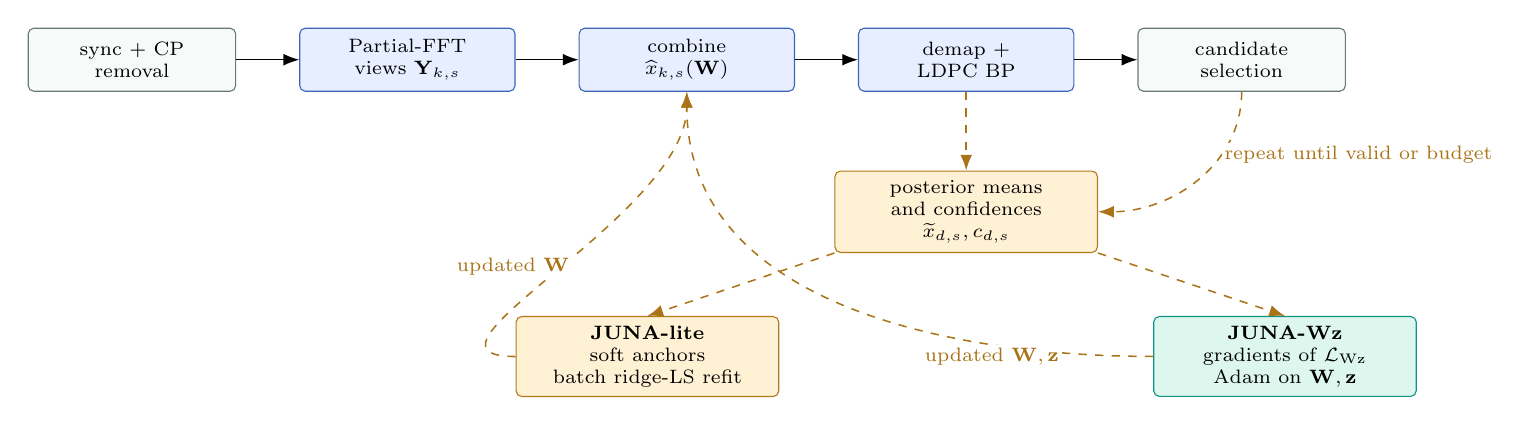
\begin{tikzpicture}[
  >=Latex,
  font=\scriptsize,
  node distance=7mm and 8mm,
  stage/.style={draw=labLine!70, rounded corners=2pt, align=center,
                fill=labPanel, minimum height=8mm, text width=24mm},
  loopstage/.style={draw=labBlue!85!black, rounded corners=2pt, align=center,
                    fill=labBlueLight, minimum height=8mm, text width=25mm},
  feedbackbox/.style={draw=labGold!90!black, rounded corners=2pt, align=center,
                      fill=labGoldLight, minimum height=8mm, text width=31mm},
  gradbox/.style={draw=labTeal!80!black, rounded corners=2pt, align=center,
                  fill=labGreenLight, minimum height=8mm, text width=31mm},
  tag/.style={fill=white, inner sep=1pt},
  arr/.style={-{Latex[length=2mm]}, line width=0.45pt},
  looparr/.style={-{Latex[length=2mm]}, dashed, color=labGold!85!black,
                  line width=0.55pt}
]
\node[stage] (sync) {sync + CP\\removal};
\node[loopstage, right=of sync] (pfft) {Partial-FFT\\views \(\mathbf Y_{k,s}\)};
\node[loopstage, right=of pfft] (eq) {combine\\\(\widehat x_{k,s}(\mathbf W)\)};
\node[loopstage, right=of eq] (bp) {demap +\\LDPC BP};
\node[stage, right=of bp] (select) {candidate\\selection};

\draw[arr] (sync) -- (pfft);
\draw[arr] (pfft) -- (eq);
\draw[arr] (eq) -- (bp);
\draw[arr] (bp) -- (select);

\node[feedbackbox, below=10mm of bp] (post) {posterior means\\and confidences\\
  \(\widetilde x_{d,s},c_{d,s}\)};
\node[feedbackbox, below left=8mm and 7mm of post] (lite) {\textbf{\junalite}\\
  soft anchors\\batch ridge-LS refit};
\node[gradbox, below right=8mm and 7mm of post] (wz) {\textbf{\junawz}\\
  gradients of \(\mathcal L_{\rm Wz}\)\\Adam on \(\mathbf W,\mathbf z\)};

\draw[looparr] (bp.south) -- (post.north);
\draw[looparr] (post.south west) -- (lite.north);
\draw[looparr] (post.south east) -- (wz.north);
\draw[looparr] (lite.west) to[out=180,in=-90]
  node[pos=0.55,below left,tag] {updated \(\mathbf W\)}
  (eq.south);
\draw[looparr] (wz.west) to[out=180,in=-90]
  node[pos=0.25,below,tag] {updated \(\mathbf W,\mathbf z\)}
  (eq.south);
\draw[looparr] (select.south) to[out=-90,in=0]
  node[pos=0.33,right,tag] {repeat until valid or budget}
  (post.east);
\end{tikzpicture}%
}
\caption{Pictorial view of the implemented \juna{} feedback loop. The receiver
first runs the ordinary Partial-FFT/FEC seed path. LDPC BP then returns
posterior soft information. \junalite{} turns reliable posterior means into
soft RLS anchors for the same Partial-FFT combiner, while \junawz{} uses the
same decoder information inside the reduced gradient loss
\(\mathcal L_{\rm Wz}\). Each refinement is decoded and scored, and the loop is
bounded by validity checks and iteration or gradient-step budgets.}
\label{fig:juna-iterative-loop}
\end{figure*}

\subsection{LDPC Decode Pass}
The same LDPC interface is used by the OFDM+FEC, Partial~FFT+FEC, and \juna{}
receivers. Its input is a scalar equalized data grid
$\widehat x_{d,s}$, not the raw waveform. First, the receiver estimates an
effective demapper scale from the outer-pilot residuals,
\begin{equation}
  \widehat\beta_{\rm LLR}
  =\max\!\left\{
    \frac{1}{SN_p}\sum_{s}\sum_{p\in\mathcal P}
      \abs{\widehat x_{p,s}-P_{p,s}}^2,\;
    \beta_{\rm floor}
  \right\},
  \label{eq:fec-sigma}
\end{equation}
with a configured floor to avoid overconfident LLRs. The quantity
$\widehat\beta_{\rm LLR}$ is an empirical LLR scale, not a physical estimate of
$N_0$: it is computed from pilot residuals and includes the constellation
normalization convention used by the demapper. For QPSK, the channel LLRs fed to
the code are
\begin{equation}
  \begin{aligned}
  L^{\rm ch}_{I,d,s}
    &=\mathrm{clip}_{L_{\max}}\!\left(
      \frac{2\Re\{\widehat x_{d,s}\}}
      {\widehat\beta_{\rm LLR}}\right),\\
  L^{\rm ch}_{Q,d,s}
    &=\mathrm{clip}_{L_{\max}}\!\left(
      \frac{2\Im\{\widehat x_{d,s}\}}
      {\widehat\beta_{\rm LLR}}\right),
  \end{aligned}
  \label{eq:qpsk-channel-llr}
\end{equation}
where positive LLR means bit zero and negative LLR means bit one. Other PSK
modulations use the analogous constellation demapper. The channel LLR vector is
deinterleaved into LDPC bit order, then inner-pilot message coordinates are
clamped to $\pm\min(L_{\max},L_{\rm ip})$ according to their known bits. These
inner pilots are code-domain constraints; they are not OFDM pilot tones and are
excluded from payload BER and PSR accounting.

The decoder then tests whether the clamped hard decision already satisfies the
parity checks. If it does, the decode returns immediately with zero BP
iterations and posterior LLRs equal to the clamped channel LLRs. Otherwise the
code runs message passing on the Tanner graph of $\Hc$. In the exact
sum-product path, check-to-variable messages are
\begin{equation}
  L_{j\to i}^{(t)}
  =2\,\operatorname{atanh}
    \prod_{i'\in\mathcal N(j)\setminus i}
    \tanh\!\left(\frac{L_{i'\to j}^{(t-1)}}{2}\right),
  \label{eq:bp-check}
\end{equation}
and variable-to-check messages add the channel LLR and all other incoming check
messages,
\begin{equation}
  L_{i\to j}^{(t)}
  =L_i^{\rm ch}+
   \sum_{j'\in\mathcal M(i)\setminus j}L_{j'\to i}^{(t)} .
  \label{eq:bp-var}
\end{equation}
The posterior returned to the receiver is
$L_i^{\rm post}=L_i^{\rm ch}+\sum_{j\in\mathcal M(i)}L_{j\to i}$. The profiled
workbench runs use the faster normalized min-sum approximation: each check sends
the product of incoming signs times the smallest excluded magnitude, scaled by
$\alpha_{\rm MS}=0.8$. Both variants hard-decide $b_i=1$ when
$L_i^{\rm post}<0$, test the syndrome after each configured check period, and
stop early when all checks pass. Thus the decoder returns three objects used by
\juna{}: hard decoded bits for BER/validity, a syndrome-valid flag, and the
posterior LLR vector that becomes soft equalizer-training information.

\subsection{\texorpdfstring{\junalite{}}{JUNA-lite}: Posterior Means as Soft Data
Anchors}\label{ssec:junalite}
The lightweight variant approximates the reduced code-aware update without
forming a gradient.
For QPSK, posterior LLRs map to posterior means and a confidence
\begin{equation}
  \begin{aligned}
  \widetilde x_{d,s}
    &=\tfrac{1}{\sqrt2}\big(\tanh\tfrac{L_{I}}{2}
      +j\tanh\tfrac{L_{Q}}{2}\big),\\
  c_{d,s}
    &=\min\!\big(\abs{\tanh\tfrac{L_{I}}{2}},
      \abs{\tanh\tfrac{L_{Q}}{2}}\big),
  \end{aligned}
  \label{eq:qpsk-posterior}
\end{equation}
with the corresponding one-dimensional posterior mean for BPSK.
\junalite{} forms the anchor set $\mathcal A_b=\mathcal P_b\cup\{(d,s):d\in b,\,
c_{d,s}\ge c_{\min}\}$ with $\abs{\mathcal A_b\setminus\mathcal P_b}\le A_{\max}$,
and reruns the same batch ridge-LS update with desired responses equal to the known pilots
on $\mathcal P_b$ and the posterior means $\widetilde x_{k,s}$ on the selected
data anchors. The default package receiver therefore trains toward posterior
means---not hard decisions---keeps pilots in the anchor set, and can reject a
refinement. Pilot rows have unit weight and selected data rows use $c_{d,s}$ as
their row weight. JunaCore sets $c_{\min}=0$, leaves $A_{\max}$ effectively
unbounded, and allows two refinement passes. A threshold and finite cap remain
testable internal controls. The ReplayCh measured profile instead uses recursive
RLS and a finite cap, as recorded separately in Table~\ref{tab:hyperparams}.

\begin{algorithm}[t]
\caption{\junalite{} posterior-anchor batch ridge-LS refinement}
\label{alg:junalite}
\footnotesize
\begin{algorithmic}[1]
\Require Partial-FFT views, pilots, LDPC code, budgets \(I_{\max},A_{\max}\),
  threshold \(c_{\min}\)
\State Train/apply the pilot-only Partial-FFT ridge-LS seed.
\State Demap to channel LLRs, run LDPC BP, and store the seed candidate.
\For{\(i=1,\ldots,I_{\max}\)}
  \State Map posterior LLRs to \(\widetilde x_{d,s}\) and \(c_{d,s}\).
  \For{each frequency band \(b\)}
    \State Build \(\mathcal A_b\) from pilots and confident data anchors.
    \State Refit the band combiner with unit pilot and confidence-weighted data rows.
  \EndFor
  \State Equalize with the updated \(\mathbf W\) and demap to LLRs.
  \State Decode and score the candidate by Section~\ref{ssec:solver-selection}.
  \State Keep the best candidate under validity, syndrome, and score tests.
  \If{the candidate is accepted or the budget is exhausted}
    \State \textbf{break}
  \EndIf
\EndFor
\State \Return the best decoder-grounded candidate.
\end{algorithmic}
\end{algorithm}

\subsection{Candidate Selection}\label{ssec:candidate-selection}
\label{ssec:solver-selection}
Each pass decodes the candidate symbols and compares decoder-first. In strict
mode, a valid LDPC codeword beats an invalid one, and lower syndrome weight
breaks ties; remaining ties use a score combining pilot MSE,
confidence-weighted distance from equalized symbols to posterior means over the
data grid,
normalized syndrome weight, and a small reward for sharper posteriors:
\begin{equation}
  S_{\rm cand}
  =M_{\rm pilot}+0.25\,M_{\rm tie}
   +0.05\,w_{\rm synd}-10^{-4}\overline{|L^{\rm post}|}.
  \label{eq:candidate-score}
\end{equation}
Here
\begin{equation}
  M_{\rm pilot}
  =\frac{1}{SN_p}\sum_{s}\sum_{p\in\mathcal P}
    \abs{\widehat x_{p,s}-P_{p,s}}^2,
  \label{eq:candidate-pilot-mse}
\end{equation}
and, for QPSK,
\begin{equation}
  M_{\rm tie}
  =\frac{\sum_{s}\sum_{d\in\mathcal D}\max(c_{d,s},10^{-3})
          \abs{\widehat x_{d,s}-\widetilde x_{d,s}}^2}
         {\sum_{s}\sum_{d\in\mathcal D}\max(c_{d,s},10^{-3})}.
  \label{eq:candidate-tie-mse}
\end{equation}
Other modulations use the same weighted tie MSE after mapping LLRs to
constellation posterior means. The term $w_{\rm synd}$ is the syndrome weight
divided by the number of parity checks, and
$\overline{|L^{\rm post}|}$ is the mean posterior-LLR magnitude. Lower
$S_{\rm cand}$ is better only after the decoder-first validity and syndrome
tests above, so the scalar score does not override a valid codeword with an
invalid one. The profiled replay runs enable a second, CRC-surrogate mode: the
harness declares a packet accepted when the recovered unknown payload bits
exactly match the transmitted payload, even if the LDPC syndrome flag is not set.
This replay-only surrogate emulates an ideal payload CRC for acceptance
accounting and early exit; it is not used to form posterior anchors or to change
the non-oracle score in~\eqref{eq:candidate-score}. In a deployed packet format,
the known-payload check would be replaced by a real CRC or by strict
syndrome/score selection. Strict-syndrome validity and the non-oracle score above
are recorded separately.

At the public package boundary, \texttt{Modulations.demodulate} returns
soft bit metrics and a CFO estimate. It does not expose a CRC-backed packet-valid flag.
Validity, syndrome weight, and candidate score are internal ordering signals;
payload-exact matching belongs only to the offline replay evaluation harness.

\subsection{\texorpdfstring{\junawz{}}{JUNA-Wz}: Confidence-Weighted
Descent}\label{ssec:gradient-juna}
\junawz{} is the deployed gradient receiver. It does not optimize the full
$(\mathbf W,\mathbf C,\mathbf z)$ objective; instead it freezes the explicit
ICI/partial-FFT-domain response tensor and descends a reduced loss over the partial-FFT
combiner and QPSK bit logits. Let
$\widehat x_{k,s}(\mathbf W)=\mathbf w_{b(k),s}\Ht\mathbf Y_{k,s}$ be the
bandwise combiner output and $s_{k,s}(\mathbf z)$ be the relaxed symbol implied
by the bit logits. The reduced loss has the form
\begin{equation}
  \begin{aligned}
  \mathcal L_{\rm Wz}(\mathbf W,\mathbf z)
  ={}&
  \alpha_p\sum_s\sum_{p\in\mathcal P}
       \abs{\widehat x_{p,s}(\mathbf W)-P_{p,s}}^2\\
  &+\alpha_t\sum_s\sum_{d\in\mathcal D}
       c_{d,s}\abs{\widehat x_{d,s}(\mathbf W)-s_{d,s}(\mathbf z)}^2\\
  &+\lambda_{\rm p}\mathcal R_{\rm par}(\mathbf z)
   +\eta_W\norm{\mathbf W-\mathbf W_0}_F^2\\
  &+\gamma_z\norm{\mathbf z}_2^2
   +\frac{\mu}{2}\norm{\mathbf z-\mathbf z_0}_2^2 .
  \end{aligned}
  \label{eq:gradient-rescue}
\end{equation}
The seed $(\mathbf W_0,\mathbf z_0)$ comes from the partial-FFT/\junalite{}
candidate and its channel or posterior LLRs, $\mu$ is a trust weight to prevent
large moves away from the seed, and
$\mathcal R_{\rm par}(\mathbf z)$ is~\eqref{eq:soft-parity} with
$\xi_i=\tanh(z_i/2)$. The implementation evaluates analytic gradients of the
combiner residuals, QPSK posterior-mean map, parity product penalty, $\ell_2$
regularizer, and trust term, then applies Adam updates to $\mathbf W$ and
$\mathbf z$. Each data coordinate is weighted by the decoder confidence
$c_{d,s}$ of~\eqref{eq:qpsk-posterior}, so informative symbols pull harder than
uncertain ones. BP projection is not applied inside Adam: after each parameter
step, the state is converted to soft metrics, decoded, and compared with the
best candidate under the non-oracle ordering of
Section~\ref{ssec:candidate-selection}. The best finite objective checkpoint is
also decoded once at the end. \junalite{}
(Section~\ref{ssec:junalite}) is the cheaper approximation that carries the
at-scale sweeps.

\begin{algorithm}[t]
\caption{\junawz{} robust reduced-gradient refinement}
\label{alg:junawz}
\footnotesize
\begin{algorithmic}[1]
\Require Partial-FFT views, pilots, LDPC checks, seed
  \((\mathbf W_0,\mathbf z_0)\), confidences \(c_{d,s}\), step budget \(G=20\)
\State Initialize \((\mathbf W,\mathbf z)\gets(\mathbf W_0,\mathbf z_0)\).
\State Store the seed or \junalite{} candidate as the current best.
\For{\(g=1,\ldots,G\)}
  \State Form \(\widehat x_{k,s}(\mathbf W)\) and relaxed symbols
    \(s_{k,s}(\mathbf z)\).
  \State Evaluate \(\mathcal L_{\rm Wz}(\mathbf W,\mathbf z)\) in
    \eqref{eq:gradient-rescue}.
  \State Compute analytic gradients with respect to \(\mathbf W\) and
    \(\mathbf z\).
  \State Take one Adam step, including trust and regularization terms.
  \State Map \(\mathbf z\) to soft metrics, run BP, and update the best candidate.
\EndFor
\State Decode the best-loss checkpoint once more if needed.
\State \Return the best decoder-grounded candidate.
\end{algorithmic}
\end{algorithm}

\subsection{\texorpdfstring{\junawcz{}}{JUNA-WCz}: A Constrained Coupled
Receiver}\label{ssec:juna-wcz}
\junawcz{} updates the full $(\mathbf W,\mathbf C,\mathbf z)$ triple of
\eqref{eq:juna-total}---the partial-FFT combiner $\mathbf W$, a banded
partial-FFT-domain ICI tensor $\mathbf C$, and the QPSK bit logits $\mathbf z$---with
joint Adam steps. An early diagnostic prototype descended the unconstrained
per-carrier objective; because those extra $\mathbf C$ degrees of freedom are
numerous and only weakly identifiable from sparse pilots
(Section~\ref{ssec:juna-objective}), the prototype served purely as a sanity
check that opening the full objective moves the same decoder metrics in the same
direction on a controlled segment.

Table~\ref{tab:full-gradient-check} reports a same-segment comparison on the
current native \texttt{red\_1} QPSK profile: receiver~1, replay time
$0$--$4$\,s, and 30\,dB SNR. The comparison uses the same 11 packets and
disables the usual non-regression gate, so the \junawcz{} row is the raw
optimizer output rather than ``best of \junalite{} and \junawcz{}.'' With an
eight-step gradient budget and ICI half-bandwidth
$K_{\rm ICI}=1$, the full-objective optimizer matches \junalite{} on valid
packet count ($1/11$ for both) and differs by only two message-bit errors out of
$7491$. This single segment is a diagnostic sanity check, not a replacement for
the measured-channel mirrors of Section~\ref{sec:results}; we read it as
evidence that opening the full objective does not degrade decoder metrics on a
controlled stress segment, not as a \junawcz{} win over \junalite{}.

The deployed \junawcz{} receiver replaces the unconstrained prototype with a
frozen, testable scope: QPSK, one OFDM symbol per solve, ICI half-width
$K{=}1$, and both $\mathbf W$ and $\mathbf C$ tied across the $B$ frequency
bands of the front end, with inner-pilot logits hard-clamped, filler symbols
fixed and known, the DC carrier excluded, and out-of-band neighbors
contributing zero. Its objective is~\eqref{eq:juna-total} under this
band-tied parameterization with $\Sigma_k=\sigma^2\mathbf I$:
\begin{equation}
  \mathcal L_{\mathrm{bt}}(\mathbf C,\mathbf W,\mathbf z)
  =\sum_{f\in\mathcal F} w_f\,\overline{L}_f(\mathbf C,\mathbf W,\mathbf z),
  \qquad
  \mathbf c_{k,q}=\mathbf c_{b(k),\,q-k},
  \label{eq:juna-wcz}
\end{equation}
where $\mathcal F$ ranges over the seven families
of~\eqref{eq:juna-total}, each $\overline{L}_f$ is normalized by its own
number of scalar contributions so the weights $w_f$ keep their meaning across
geometries, and $b(k)$ is the band index of carrier $k$. By the counting
argument of Section~\ref{ssec:juna-objective}, the band-tied fit is
overdetermined whenever a band holds more than $2K{+}1$ carriers, so the
observation family disciplines $\mathbf z$ instead of being absorbed by free
response coefficients.

The runtime family-weight tuple is
\texttt{(1.0,2.0,0.1,0.002,0.02,0.02,0.08)} for observation, pilot, tie,
$\mathbf C$ regularization, $\mathbf W$ regularization, smoothness, and parity,
respectively. JunaCore takes eight public joint-Adam steps with hand-derived
Wirtinger gradients; the public logit step is $\alpha_z=0.004$, on the same
scale as the response update, to avoid overshooting a decoder-better early
logit state. BP projection is not applied inside Adam; BP is used only
when the optimized state is turned into a receiver candidate. A safeguarded
block-coordinate implementation is an internal reference optimizer for testing
the same constrained objective, not a fourth public receiver profile.

Initialization is deterministic: $\mathbf W_0$ is the pilot-trained combiner
of~\eqref{eq:pfft-ls}, $\mathbf z_0$ clamps the seed posterior LLRs (with
known inner-pilot bits pinned at the clamp rail), and $\mathbf C_0$ is a
bandwise ridge profile of the observations given the relaxed symbols
$s(\mathbf z_0)$. The solver takes a fixed budget of joint Adam steps on
hand-derived Wirtinger gradients, re-clamps inner-pilot logits after every
step, and retains the best finite objective checkpoint, so optimization can
never worsen its own scalar objective
(Algorithm~\ref{alg:junawcz}). The optimized state re-enters the decoder
boundary exactly as the other receivers do: the best $\mathbf W$ equalizes the
carriers, the negated logits become clipped soft metrics, BP scores the
candidate, and the validity/syndrome/score ordering of
Section~\ref{ssec:candidate-selection} keeps the seed unless the coupled
candidate genuinely improves it.

\begin{algorithm}[t]
\caption{\junawcz{} constrained joint refinement}
\label{alg:junawcz}
\footnotesize
\begin{algorithmic}[1]
\Require Partial-FFT views, pilots, LDPC checks, seed candidate, step budget
  \(T\)
\State Initialize \(\mathbf W_0\) from the pilot-trained combiner and
  \(\mathbf z_0\) from clamped seed posteriors; pin inner-pilot logits.
\State Profile \(\mathbf C_0\) by bandwise ridge regression of the
  observations on the relaxed symbols \(s(\mathbf z_0)\).
\For{\(t=1,\ldots,T\)}
  \State Evaluate \(\mathcal L_{\mathrm{bt}}\) in~\eqref{eq:juna-wcz} and its
    analytic Wirtinger gradients in \((\mathbf C,\mathbf W,\mathbf z)\).
  \State Take one clipped joint Adam step; re-clamp inner-pilot logits.
  \State Retain the best finite objective checkpoint seen so far.
\EndFor
\State Equalize with the best \(\mathbf W\); map \(-\mathbf z\) to clipped
  soft metrics; BP-score the candidate.
\State \Return the candidate iff it improves the seed under the
  validity/syndrome/score order; otherwise the seed.
\end{algorithmic}
\end{algorithm}

Table~\ref{tab:wcz-ici} reports the controlled residual-ICI stress that the
deployed receiver is regression-tested against: one 1024-tone block carrying
170 payload bits is rotated by a residual frequency offset of $0.08$
subcarrier spacings (creating ICI without invoking the optional sync/CFO
correction) and decoded under seeded AWGN. At 3\,dB and above the seed is already
valid and the non-regression gate keeps it. At 0\,dB the coupled candidate is
accepted and improves both the syndrome weight ($208\to105$) and the true
payload error count ($33\to31$). The 1.5\,dB row documents a property of
proxy-based selection that we consider important to state explicitly: the
acceptance ordering compares validity, syndrome, and score---quantities the
receiver can compute without ground truth---and at this operating point it
accepts a candidate whose syndrome is lower ($129\to83$) while its true
payload error count is one bit higher ($18\to19$). The same behavior class was
observed for the coupled acceptance rule in the offline replay experiments;
strict LDPC validity and payload-exact acceptance are therefore tracked
separately throughout Section~\ref{sec:results}.

\begin{table}[t]
\centering
\caption{Controlled residual-ICI stress for the deployed \junawcz{} receiver:
$0.08$-subcarrier CFO plus seeded AWGN, one 1024-tone block, 170 payload
bits, eight Adam steps. ``Accepted'' means the coupled candidate replaced the
seed under the validity/syndrome/score ordering.}
\label{tab:wcz-ici}
\small
\begin{tabular}{lccccc}
\toprule
SNR (dB) & Seed synd. & \junawcz{} synd. & Seed err. & \junawcz{} err. &
Accepted \\
\midrule
12.0 & 0   & --- & 0  & --- & no (seed valid) \\
3.0  & 0   & --- & 0  & --- & no (seed valid) \\
1.5  & 129 & 83 & 18 & 19  & yes \\
0.0  & 208 & 105 & 33 & 31  & yes \\
\bottomrule
\end{tabular}
\end{table}

Every component of the deployed receiver is pinned by an executable contract
in the accompanying test harness: the seven objective families are checked
term-by-term against independently hand-computed fixtures, the analytic
Wirtinger gradients against exhaustive centered finite differences over every
coordinate, the band-tied observation term against a discrimination test that
verifies it prefers the true bits over corrupted bits (and an
overdetermination guard that fails if the band geometry regresses to the
underdetermined per-carrier form), and the public receiver against the same
interface, robustness, and acceptance contracts as \junalite{} and
\junawz{}.

\begin{table}[t]
\centering
\caption{Raw \junalite{} versus diagnostic \junawcz{} on the same
\texttt{red\_1} segment.}
\label{tab:full-gradient-check}
\small
\resizebox{\columnwidth}{!}{%
\begin{tabular}{lccccc}
\toprule
Method & Msg. errors & Msg. bits & Msg. BER & Code BER & Valid pkts. \\
\midrule
\junalite{} (posterior-anchor) & 34 & 7491 & $4.539{\times}10^{-3}$ & $1.490{\times}10^{-2}$ & 1/11 \\
\junawcz{} $(\mathbf W,\mathbf C,\mathbf z)$ & 32 & 7491 & $4.272{\times}10^{-3}$ & $1.379{\times}10^{-2}$ & 1/11 \\
\bottomrule
\end{tabular}
}
\\[2pt]
\footnotesize Receiver 1, \texttt{red\_1}, $0$--$4$\,s, 30\,dB, 11 packets,
$N=1536$, CP $=4$, one symbol, pilot spacing $3$, rate $1/3$, $d_{\rm cfg}=7$,
gradient steps $=8$, $K_{\rm ICI}=1$. The hard-decision pre-BP BERs are
$8.419{\times}10^{-2}$ and $8.388{\times}10^{-2}$, respectively.
\end{table}

\subsection{Why It Helps, and Three Regimes}
If posterior anchors were independent unbiased observations, enlarging the
training set would reduce the variance of the ridge-LS estimate,
$\operatorname{Cov}(\widehat{\mathbf w}_b)\approx\sigma^2(\mathbf
Y_{\mathcal A_b}\Ht\mathbf Y_{\mathcal A_b}+\delta I)^{-1}$. This is intuition,
not proof: the anchors are decoder-processed functions of the same noisy seed and
are correlated with it. The gain therefore comes from adding correlated but
shrunken constraints that are useful when the posterior is informative; the
danger is posterior bias, guarded by posterior means (not hard slices),
anchor caps, retained pilots, validity/syndrome selection, and
early stopping. This leads to three empirical regimes: on easy channels Partial~FFT
already decodes and \juna{} ties; on impossible channels the seed posterior is
uninformative and \juna{} cannot help; on hard-but-decodable channels the
posterior is informative but not decisive, and posterior anchors can move the
re-decode across the success boundary. The extra cost is bounded for the
deployed receivers: a fixed number of \junawz{} gradient steps or \junalite{}
ridge-LS refits, plus decoder-grounded BP checks.

%=============================================================================
\section{Computational Complexity}\label{sec:complexity}
This section counts one decoded frame, since the replay experiments apply the
same waveform schedule to all receivers. Let $N$ be the FFT size, $S$ the number
of OFDM data symbols in a frame, $N_a$ the number of active subcarriers, $N_p$
the number of outer pilot tones, and $N_d=N_a-N_p$ the number of data tones. Let
$N_{\rm view}$ be the number of partial-FFT views, $B$ the number of frequency
bands, $A\le A_{\max}$ the selected posterior data anchors per symbol, and
$I\le I_{\max}$ the number of \juna{} refinement passes actually executed after
early stopping. For \junawz{}, let $G$ be the number of Adam steps in one
gradient refinement and $C_{\rm cand}$ the number of BP candidate decodes during
that descent. For \junawcz{}, let $K$ be the ICI half-band used in
the partial-FFT-domain response tensor. For the LDPC code, let $n_b=k+m$ be the codeword length, $E$ the
number of Tanner-graph edges, and $T_{\rm BP}$ the number of BP/min-sum
iterations used by a decode attempt.

\subsection{Common OFDM and LDPC Costs}
The one-tap OFDM receiver performs packet synchronization, CP removal, an
$N$-point FFT per OFDM symbol, pilot interpolation, symbol demapping, and one
LDPC decode. The FFT term is $O(SN\log N)$. Pilot interpolation and one-tap
equalization are linear in the active grid, $O(SN_a)$. The implemented LDPC
decoder first checks hard parity and otherwise runs belief propagation or
normalized min-sum. Both variants pass messages along Tanner edges, so the
decode cost is
\begin{equation}
  T_{\rm LDPC}=O(T_{\rm BP}E),
  \label{eq:ldpc-complexity}
\end{equation}
with early stopping reducing the realized iteration count. Since the systematic
matrix is sparse, code construction and encoding are one-time per configuration
costs outside the online receive loop; their storage and arithmetic scale with
the same sparse edge count.

\subsection{Partial-FFT Linear-Combiner Front End}
The Partial~FFT+FEC receiver replaces each active FFT coefficient by
$N_{\rm view}$ partial-FFT views. In the profiled implementation, each view is
formed by zeroing the other short-time windows and applying the same
$N$-point FFT plan; therefore the implemented
partial-FFT extraction cost is
\begin{equation}
  T_{\rm pfft}=O(SN_{\rm view}N\log N).
  \label{eq:pfft-cost}
\end{equation}
A shorter transform could reduce this constant, but that is not the receiver
benchmarked here. A bandwise linear-combiner fit processes length-$N_{\rm view}$
rows from the outer pilots. Either ReplayCh's recursive update or JunaCore's
batch normal-equation accumulation costs
$O(N_{\rm view}^2)$ per row; the package additionally solves one
$N_{\rm view}\times N_{\rm view}$ system per band. Training therefore costs
$O(SN_pN_{\rm view}^2)$, while applying the learned combiner to all active bins costs
$O(SN_aN_{\rm view})$. The Partial~FFT+FEC receiver thus has online cost
\begin{equation}
  T_{\rm PF}
  =O(SN_{\rm view}N\log N+SN_pN_{\rm view}^2+SN_aN_{\rm view}+T_{\rm BP}E).
  \label{eq:pf-complexity}
\end{equation}
For the ReplayCh reported runs, $N_{\rm view}=4$ and $B=4$; JunaCore uses four
views and $B=16$. In both cases the matrices are small, and the main cost
increase over one-tap OFDM is the fixed number of extra FFT views plus the LDPC
decode shared by all FEC receivers.

\subsection{Per-Pass Refinement Cost}
Both \junalite{} and \junawz{} start from the Partial~FFT+FEC seed and run a bounded
number of passes. \junalite{} converts LDPC posterior LLRs into soft symbols,
selects data anchors, refits the same bandwise batch ridge-LS combiner using pilots plus
anchors, applies the combiner, and decodes the candidate. Posterior-to-symbol
conversion is linear in the data
grid, $O(SN_d)$. When all QPSK data anchors are used, anchor construction remains
linear. In the capped-confidence path, sorting candidates costs
$O(SN_d\log N_d)$ in the worst case, but the profiled QPSK runs use the linear
all-anchor path when $A_{\max}$ covers the data tones. The ridge-LS refit costs
$O(S(N_p+A)N_{\rm view}^2)$, combiner application costs $O(SN_aN_{\rm view})$, phase/pilot residual
correction and candidate scoring are linear in the active grid, and the candidate
decode costs another $O(T_{\rm BP}E)$. Hence
\begin{equation}
\begin{aligned}
  T_{\juna}
  ={}& T_{\rm PF}
  + I\,O\big(T_{\rm BP}E+SN_d+S(N_p+A)N_{\rm view}^2\\
  &\hspace{2.7em}+SN_aN_{\rm view}+SN_a\big),
\end{aligned}
  \label{eq:juna-complexity}
\end{equation}
plus the optional $O(ISN_d\log N_d)$ sorting term when the confidence-capped path
is active. This is a bounded constant-factor extension of Partial~FFT+FEC under
the respective settings. ReplayCh uses $I_{\max}=4$, $A_{\max}=1024$,
$N_{\rm view}=4$, and $B=4$ for the measured profile; JunaCore uses
$I_{\max}=2$, no finite default anchor cap, $N_{\rm view}=4$, and $B=16$.
Easy package packets terminate immediately when the seed is valid, and every
path pays at most its fixed iteration budget.

\junawz{} replaces the ridge-LS refit with $G$ Adam steps on
\eqref{eq:gradient-rescue}. One step evaluates combiner outputs and their
gradients over the active partial-FFT grid, maps logits to QPSK soft symbols, and
evaluates the soft-parity gradient over Tanner edges. Its reduced-gradient
increment is therefore
\begin{equation}
\begin{aligned}
  T_{\rm Wz}
  ={}&T_{\rm PF}
   +O\!\big(G(SN_aN_{\rm view}+SN_d+E)\\
   &\hspace{2.2em}+(C_{\rm cand}+1)T_{\rm BP}E\big),
\end{aligned}
  \label{eq:wz-complexity}
\end{equation}
where the extra decode covers the final best-loss state when it is not already
the best candidate. With fixed $G$ and
small $N_{\rm view}$, this is also a bounded online extension of Partial~FFT+FEC,
but with a larger constant than \junalite{}.

\junawcz{} is more expensive because every step additionally evaluates and
updates a partial-FFT-domain response tensor with $(2K+1)$ carrier offsets:
\begin{equation}
  T_{\rm WCz}
  =T_{\rm PF}
   +O\!\left(G_{\rm full}(SN_a(2K+1)N_{\rm view}+SN_d+E)\right).
  \label{eq:wcz-complexity}
\end{equation}
Its memory includes $O(SBN_{\rm view}(2K+1))$ complex $\mathbf C$ coefficients in
addition to $\mathbf W$ and the logits. This path is therefore reported as a
diagnostic solver, not as the computationally inexpensive receiver used for the
large measured-channel sweeps.

\begin{table}[t]
\centering
\caption{Dominant online per-frame receiver complexity.}
\label{tab:complexity}
\small
\resizebox{\columnwidth}{!}{%
\begin{tabular}{@{}lp{0.68\columnwidth}@{}}
\toprule
Branch & Dominant cost \\
\midrule
OFDM+FEC &
$O(SN\log N+SN_a+T_{\rm BP}E)$ \\
Partial~FFT+FEC &
$O(SN_{\rm view}N\log N+SN_pN_{\rm view}^2+SN_aN_{\rm view}+T_{\rm BP}E)$ \\
\junalite{}+FEC &
$T_{\rm PF}+I\,O(T_{\rm BP}E+SN_d+S(N_p+A)N_{\rm view}^2+SN_aN_{\rm view}+SN_a)$ \\
\junawz{}+FEC &
$T_{\rm PF}+O(G(SN_aN_{\rm view}+SN_d+E)+(C_{\rm cand}+1)T_{\rm BP}E)$ \\
\junawcz{}+FEC &
$T_{\rm PF}+O(G(SN_a(2K{+}1)N_{\rm view}+SN_d+E)+T_{\rm BP}E)$ \\
\bottomrule
\end{tabular}
}
\end{table}

\subsection{Memory and Offline Search}
The one-tap receiver stores the active symbol grid, channel estimates, and LDPC
messages, giving $O(SN_a+E)$ receiver memory. Partial~FFT stores the partial-FFT
observations, $O(SN_{\rm view}N_a)$, plus bandwise weights and small normal-equation state,
$O(BN_{\rm view}+BN_{\rm view}^2)$. \juna{} adds the current/best equalized candidates and posterior
LLRs, $O(SN_a+n_b)$, but reuses the LDPC scratch buffers and combiner state across
passes. Thus the additional memory over Partial~FFT+FEC is linear in the frame
and codeword size, not quadratic in the subcarrier count.

Configuration search is offline. If $C$ candidate configurations are evaluated
over $R$ replay captures and $Q$ SNR points, the brute-force search cost is
$O(CRQ\,T_{\juna})$ for the JUNA-ranked sweeps, with smaller constants for
receivers that omit refinement. The coordinate and one-at-a-time (OAT) sweeps in
Section~\ref{sec:transfer} are therefore tuning procedures, not deployed
per-packet receiver operations.

%=============================================================================
\section{Experimental Method}\label{sec:method}
We evaluate three receivers on the same transmitted schedule, channel replay, SNR,
FEC, and acceptance rule: \textbf{OFDM+FEC} (one-tap pilot-linear equalization),
\textbf{Partial~FFT+FEC} (bandwise partial-FFT RLS combining), and
\textbf{\junalite{}+FEC} (partial-FFT seed, posterior extraction,
posterior-anchor RLS refinement, re-decode, candidate selection; the lightweight
\juna{} that carries the sweeps). Packet success rate (PSR) is
accepted packets over the scheduled replay packets entering the common decoding
pipeline; the schedules are shared across receivers, and receiver-specific
non-acceptance remains in the denominator. In these offline replay experiments,
acceptance is payload-exact recovery, which is used as an idealized stand-in for
the payload CRC available in a deployed packet format. This acceptance rule is
applied uniformly to all receivers; strict LDPC validity is tracked separately but
is not the headline PSR rule. BER is pooled post-FEC payload-message BER after
the receiver's selection rule, excluding inner-pilot message bits. Goodput is
\begin{equation}
  G=\frac{N_{\rm acc}k_{\rm payload}}{T_{\rm replay}},
  \label{eq:goodput}
\end{equation}
where $N_{\rm acc}$ is the number of accepted packets, $k_{\rm payload}$ excludes
inner-pilot message bits, and $T_{\rm replay}$ is the replay time spanned by the
scheduled packets. Reported PSR uncertainty uses Wilson 95\% binomial intervals
computed from the accepted/decoded packet counts.
Configuration search is brute force over a finite candidate pool ranked by a
lexicographic tuple
$(\mathrm{PSR},\text{goodput},\text{accepted},\text{payload bits},
-\text{decode time})$; there is no learned loss. Table~\ref{tab:hyperparams}
lists the benchmark-run hyperparameters. The exact controlled and native
benchmark table rows are also archived with this draft as
\texttt{paper/joe/benchmark\_results.csv}; the cross-channel tuning tables are
generated from the reproduction pipeline in \texttt{tex/figure\_data/}.

The measured data are replay-channel captures stored as \texttt{red},
\texttt{blue}, and \texttt{yellow} files and mapped in Section~\ref{sec:transfer}
to SG/NA/HW sites. For each packet the transmitter generates a known preamble,
outer OFDM pilot tones, data tones carrying the LDPC-coded payload, and optional
inner-pilot message bits. The clean passband packet is replayed through the same
measured channel segment for all receiver variants; AWGN is then added before
synchronization, CP removal, demodulation, and decoding. The implemented SNR is
the ratio of average clean replayed passband sample power,
$N_x^{-1}\sum_n |x[n]|^2$,
to added real passband noise power over the packet waveform passed to the
receiver. Noise seeds are deterministic functions of the packet and SNR index
unless a sweep explicitly changes them. Thus OFDM+FEC, Partial~FFT+FEC, and
\junalite{}+FEC differ only in the receiver processing after the common noisy
replay waveform. The constrained \junawcz{} receiver is evaluated on the
controlled residual-ICI and synthetic-channel experiments of
Section~\ref{ssec:juna-wcz} and on single measured segments; it does not yet
enter the full replay benchmark sweeps below, and the PSR/goodput tables should
not be read as covering it.

ReplayCh configuration identifiers encode the workbench modem geometry and code. For example,
\cfg{n1024\_cp256\_sym1\_p3\_r0p25\_dc4\_sig1\_ip2} means
$N=1024$, CP length $256$, one OFDM payload symbol per frame, one outer pilot
every three active subcarriers, LDPC design rate $0.25$, LDPC sparsity knob
$d_{\rm cfg}=4$ (encoded in the suffix as \cfg{dc4}), FEC LLR scale floor $1$,
and one inner-pilot message bit every two message positions. For the
cross-channel tuning table, the coordinate search at 20\,dB sweeps FEC rate,
outer/inner pilot spacing, $d_{\rm cfg}$, the joint $(N,\mathrm{CP})$ grid, and
modulation, fixing each stage's best JUNA PSR (with BER as the tie-breaker)
before moving to the next stage. The OAT table then perturbs one factor at a
time around a cold default to measure coarse local sensitivity; it is used as a
tuning screen, not as a causal ranking when factors tie. Table~\ref{tab:search-pool}
lists the pool used by these coordinate/OAT screens; the controlled benchmark
uses the separate robust configuration stated in Section~\ref{sec:results}.

Operationally, this paper calls a channel \emph{ceiling} when Partial~FFT+FEC is
already above roughly $0.95$ PSR, \emph{floor} when all receivers remain near zero
packet acceptance or the seed posterior is effectively uninformative, and
\emph{hard-but-decodable} when the Partial~FFT seed produces useful posterior
confidence but still fails payload acceptance on a substantial fraction of
packets. These labels are empirical regime descriptors, not pre-deployment
classifiers.

\begin{table}[t]
\centering
\caption{Finite candidate pool used by the cross-channel coordinate and OAT
tuning screens.}
\label{tab:search-pool}
\small
\begin{tabular}{lp{0.58\columnwidth}}
\toprule
Knob & Candidate values \\
\midrule
FEC rate & $\{0.25,0.5,0.75\}$ \\
Outer/inner pilot ratios & coordinate: $\{0.10,0.15,0.20\}^2$; OAT:
$\{1/4,1/5,1/7,1/10\}$ \\
$d_{\rm cfg}$ & $\{6,8,10\}$ \\
$(N,\mathrm{CP})$ & $\{512,1024,2048\}\times\{0,16,32,64,128\}$ \\
Modulation & QPSK, 8PSK \\
Cold default & $N=2048$, CP $=64$, outer/inner $=1/4$, FEC $=0.25$,
$d_{\rm cfg}=8$, QPSK \\
\bottomrule
\end{tabular}
\end{table}

\begin{table}[t]
\centering
\caption{Receiver hyperparameters for the separate ReplayCh profiled benchmark runs.}
\label{tab:hyperparams}
\small
\resizebox{\columnwidth}{!}{%
\begin{tabular}{ll}
\toprule
Component & Value \\
\midrule
Partial-FFT windows & 4 temporal views \\
Partial-FFT RLS bands & 4 frequency bands (unless config states otherwise) \\
RLS forgetting / ridge & $\lambda=0.98$, $\delta=10^{-2}$ \\
FEC decoder & LDPC BP, fast min-sum in profiled runs \\
BP iterations & 8 fast-LDPC, 24 BP cap \\
\junalite{} anchor threshold / cap & $c_{\min}=0$ (off), $A_{\max}=1024$ \\
\junalite{} iteration budget & 4 passes, early-stopped \\
\junawz{} head-to-head profile & \texttt{wz\_juna}, Adam, 30 steps, $\mu=50$ \\
Acceptance & payload-exact replay acceptance (packet-CRC surrogate) \\
\bottomrule
\end{tabular}
}
\end{table}

\begin{table}[t]
\centering
\caption{Executable defaults in the JunaCore reference implementation.}
\label{tab:junacore-defaults}
\small
\resizebox{\columnwidth}{!}{%
\begin{tabular}{ll}
\toprule
Component & Value \\
\midrule
OFDM / CP & $N=1024$, $N_{\rm cp}=256$ \\
Active / pilot / data tones & $1023/341/682$ (680 QPSK code-bearing, 2 filler) \\
LDPC & $(n_b,k)=(1360,340)$, \texttt{evencol}, three edges/column \\
Partial-FFT & 4 temporal views, 16 frequency bands \\
Ridge / BP & $\delta=10^{-3}$; 20 normalized-min-sum iterations, $\alpha=0.8$ \\
\junalite{} & confidence-weighted anchors, at most 2 refits \\
\junawz{} & hand-gradient Adam, 20 steps \\
\junawcz{} & $K=1$, band-tied $B=16$, hand-gradient Adam, 8 public steps, $\alpha_z=0.004$ \\
\junawcz{} family weights & $(1,2,0.1,0.002,0.02,0.02,0.08)$ \\
Public demodulation result & soft metrics and coarse-CFO estimate \\
\bottomrule
\end{tabular}
}
\end{table}

%=============================================================================
\section{Measured-Channel Results}\label{sec:results}
The SNR and stress benchmarks below run \junalite{}, the lightweight
posterior-anchor receiver, because it is cheap enough to sweep SNR, stacked
receivers, and---in Section~\ref{sec:transfer}---twelve captures; its rows are
labeled \junalite{}+FEC. Section~\ref{ssec:gradient-mirror} and the cross-channel
mirrors then report \junawz{} head-to-head against \junalite{}.

\subsection{Controlled Three-Channel Benchmark}
The controlled benchmark fixes a common robust geometry
(\cfg{n1024\_cp256\_sym1\_p3\_r0p25\_dc4\_sig1\_ip2}) and stacked receivers
$\{1,2,3\}$ over a $0{:}5{:}20$\,dB sweep, on \texttt{red\_1} (25/5\,kHz QPSK),
\texttt{blue\_1} (13/5\,kHz BPSK), and \texttt{yellow\_1} (13/5\,kHz BPSK).
Within each channel, the same waveform, FEC, and replay schedule are decoded by
the three algorithms. Table~\ref{tab:controlled20} reports
20\,dB. \junalite{}+FEC gives large gains on the hard \texttt{red\_1} and selected
\texttt{blue\_1} captures and a one-packet near-ceiling gain on \texttt{yellow\_1},
with substantially lower message BER on the rescued packets---evidence that the
rescued packets are genuinely better decoded, not merely re-thresholded.

\begin{table}[t]
\centering
\caption{Controlled red/blue/yellow benchmark at 20\,dB.}
\label{tab:controlled20}
\small
\resizebox{\columnwidth}{!}{%
\begin{tabular}{llccccc}
\toprule
Channel & Receiver & Payload-exact PSR & 95\% CI & Packets & BER & Goodput \\
\midrule
\texttt{red\_1} & OFDM+FEC & 0.049 & [0.021, 0.110] & 5/102 & 0.193 & 17.8 \\
                & Partial FFT+FEC & 0.559 & [0.462, 0.651] & 57/102 & $3.98{\times}10^{-3}$ & 202.8 \\
                & \junalite{}+FEC & \textbf{0.922} & [0.853, 0.960] & \textbf{94/102} & $\mathbf{6.34{\times}10^{-4}}$ & \textbf{334.4} \\
\addlinespace
\texttt{blue\_1} & OFDM+FEC & 0.631 & [0.538, 0.715] & 70/111 & 0.0423 & 113.8 \\
                 & Partial FFT+FEC & 0.694 & [0.603, 0.772] & 77/111 & $6.78{\times}10^{-3}$ & 125.2 \\
                 & \junalite{}+FEC & \textbf{0.982} & [0.937, 0.995] & \textbf{109/111} & $\mathbf{6.36{\times}10^{-4}}$ & \textbf{177.3} \\
\addlinespace
\texttt{yellow\_1} & OFDM+FEC & 0.982 & [0.936, 0.995] & 108/110 & $2.14{\times}10^{-4}$ & 178.5 \\
                   & Partial FFT+FEC & 0.991 & [0.950, 0.998] & 109/110 & $1.07{\times}10^{-4}$ & 180.1 \\
                   & \junalite{}+FEC & \textbf{1.000} & [0.966, 1.000] & \textbf{110/110} & \textbf{0} & \textbf{181.8} \\
\bottomrule
\end{tabular}
}
\\[2pt]
\footnotesize Goodput in bit/s. BER is pooled post-FEC payload-message BER after
selection, excluding inner pilots. CI is Wilson 95\% for payload-exact packet
success, the replay analogue of a packet-CRC pass. Bold marks the best receiver per
channel.
\end{table}

\subsection{Native-Bandwidth Five-Color Stress Test}
The second benchmark runs each color at its native high-rate profile over
$0{:}5{:}30$\,dB---a stress test closer to the goodput frontier.
Table~\ref{tab:native20} reports 20\,dB. The gain pattern is the predicted one:
large on hard-but-decodable \texttt{red\_1} ($18/190\to135/190$) and the selected
\texttt{blue\_1} ($35/110\to90/110$), near-ceiling on \texttt{yellow\_1} and
\texttt{purple\_1}, and absent on the floor channel \texttt{green}, where all
three receivers fail.

\begin{table}[t]
\centering
\caption{Native-maximum-bandwidth five-color benchmark at 20\,dB.}
\label{tab:native20}
\small
\resizebox{\columnwidth}{!}{%
\begin{tabular}{llccccc}
\toprule
Channel & Receiver & Payload-exact PSR & 95\% CI & Packets & BER & Goodput \\
\midrule
\texttt{red\_1} & OFDM+FEC & 0.000 & [0.000, 0.020] & 0/190 & 0.274 & 0 \\
                & Partial FFT+FEC & 0.095 & [0.061, 0.145] & 18/190 & $1.69{\times}10^{-3}$ & 216.7 \\
                & \junalite{}+FEC & \textbf{0.711} & [0.642, 0.770] & \textbf{135/190} & $\mathbf{2.75{\times}10^{-4}}$ & \textbf{1625.2} \\
\addlinespace
\texttt{blue\_1} & OFDM+FEC & 0.091 & [0.050, 0.159] & 10/110 & 0.178 & 97.9 \\
                 & Partial FFT+FEC & 0.318 & [0.239, 0.410] & 35/110 & $2.04{\times}10^{-3}$ & 342.5 \\
                 & \junalite{}+FEC & \textbf{0.818} & [0.736, 0.879] & \textbf{90/110} & $\mathbf{3.55{\times}10^{-4}}$ & \textbf{880.8} \\
\addlinespace
\texttt{yellow\_1} & OFDM+FEC & 0.893 & [0.831, 0.934] & 125/140 & $2.48{\times}10^{-5}$ & 1397.7 \\
                   & Partial FFT+FEC & 0.929 & [0.874, 0.961] & 130/140 & $9.93{\times}10^{-5}$ & 1453.7 \\
                   & \junalite{}+FEC & \textbf{1.000} & [0.973, 1.000] & \textbf{140/140} & \textbf{0} & \textbf{1565.5} \\
\addlinespace
\texttt{purple\_1} & all three & 1.000 & [0.975, 1.000] & 150/150 & 0 & 1616.5 \\
\addlinespace
\texttt{green} & all three & 0.000 & [0.000, 0.037] & 0/100 & ${\approx}0.50$ & 0 \\
\bottomrule
\end{tabular}
}
\\[2pt]
\footnotesize Goodput in bit/s. BER is pooled post-FEC payload-message BER after
selection, excluding inner pilots. CI is Wilson 95\% for payload-exact packet
success, the replay analogue of a packet-CRC pass.
\texttt{purple\_1}/\texttt{green} rows collapsed (identical across receivers).
\end{table}

\subsection{\texorpdfstring{\junalite{}}{JUNA-lite} Mechanism Checks}
Three single-run ablations of the \junalite{} receiver were used as sanity checks
rather than confidence-interval evidence. (i) Replacing posterior-mean anchors with
hard-decision anchors does not destroy the gain, so the essential mechanism is
decoder-derived anchoring plus decoder-grounded selection; posterior means remain
the default because they avoid committing to a hard slice. (ii) Forcing the final
refinement instead of selecting the best candidate is essentially tied, so
selection is not the sole source of the gain. (iii) Giving the Partial-FFT seed
the same LDPC decode-call budget as \junalite{}, without posterior anchors, is
numerically identical to ordinary Partial~FFT in the deterministic replay path;
this mainly rules out ``more decode calls'' as the mechanism. Multi-seed numeric
ablation tables remain future work.

\subsection{\texorpdfstring{\junawz{}}{JUNA-Wz}: Head-to-Head Mirror}
\label{ssec:gradient-mirror}\label{ssec:gradient-ablation}
\junawz{} of Section~\ref{ssec:gradient-juna} is the reduced gradient receiver
that \junalite{} approximates. We therefore mirror the headline benchmarks with
\junawz{} head-to-head against \junalite{} under the same payload-exact PSR rule.
Table~\ref{tab:grad-vs-lite} sweeps SNR on the three representative captures:
\junawz{} matches or exceeds \junalite{} at every displayed point, with the
largest margins at low SNR where the seed posterior is least decisive (SG-1
rises from $0.09$ to $0.86$ at $0$\,dB) and a climb to payload-exact $1.0$ as SNR
grows. These displayed cases are the ceiling-reaching SG-1/NA-1/HW-1 captures;
the four small non-significant regressions quantified below occur on other
near-floor NA captures. Table~\ref{tab:grad-aggregate} reports the full stacked
summary: across all $48$ capture$\times$SNR cells, \junawz{} is at least as good
as \junalite{} in $44$, strictly better with disjoint Wilson 95\% intervals in
$18$, and never significantly worse.

The gain is not an artefact of the two gradient guardrails.
Table~\ref{tab:gradient-ablation} shows that replacing the soft confidence
weighting with hard anchoring, or taking the final iterate instead of the
decoder-grounded checkpoint, leaves payload-exact PSR unchanged to within a single
packet on the representative captures---so the improvement comes from the
decoder-aided descent itself, not from confidence weighting or selection alone.
The cross-channel study of Section~\ref{sec:transfer} extends the tuning mirror
to all twelve captures; it supports the same tuning conclusions but does not
show the same PSR ceiling on every capture.

\begin{table}[t]
\centering
\caption{\junawz{} versus \junalite{}: payload-exact PSR across SNR on the
three representative captures. \textbf{Bold} marks a gradient win with disjoint
Wilson 95\% intervals (generated from
\texttt{tex/figure\_data/tab\_grad\_vs\_lite.tex}).}
\label{tab:grad-vs-lite}
\small
\resizebox{\columnwidth}{!}{\input{../../tex/figure_data/tab_grad_vs_lite.tex}}
\end{table}

\begin{table}[t]
\centering
\caption{\junawz{} versus \junalite{}: stacked payload-exact PSR summary over all
48 capture--SNR cells in the head-to-head comparison (generated from
\texttt{tex/figure\_data/tab\_grad\_aggregate.tex}).}
\label{tab:grad-aggregate}
\small
\resizebox{\columnwidth}{!}{\input{../../tex/figure_data/tab_grad_aggregate.tex}}
\end{table}

\begin{table}[t]
\centering
\caption{\junawz{} ablation against \junalite{}: payload-exact PSR for the default
soft \texttt{wz\_juna}, a hard-anchor variant, and a forced-final variant, each
against \junalite{}, on representative SG-1/NA-1/HW-1 captures at 5/10\,dB.
PSR follows the same payload-exact, post-selection definition as the main
tables; the final column gives the packet denominator.}
\label{tab:gradient-ablation}
\small
\resizebox{\columnwidth}{!}{\input{../../tex/figure_data/tab_gradient_ablation.tex}}
\end{table}

%=============================================================================
\section{Cross-Channel Tuning Study}\label{sec:transfer}
The benchmarks above fix a geometry. A practical question is which modem knobs
must be retuned first on a new measured channel. We replay twelve captures from
three physically distinct sites---Singapore harbour
(\texttt{SG-1/2/3}, shallow, 25\,kHz), North Atlantic (\texttt{NA-1/2/3},
mobile deep-water, 13\,kHz), and Hawaii (\texttt{HW-1}\,$\dots$\texttt{6}, moored
deep-water, 13\,kHz)---and, for each, run a coordinate search at 20\,dB and
one-factor-at-a-time (OAT) sensitivity sweeps at 10/20/30\,dB. Fig.~\ref{fig:cir}
shows a representative measured CIR per site. This is a tuning-screen study, not
a train-on-one/test-on-another transfer protocol.

\begin{figure}[t]\centering

\includegraphics[width=\linewidth]{cir_SG1_heatmap.png}\\[-1pt]

\includegraphics[width=\linewidth]{cir_NA1_heatmap.png}\\[-1pt]

\includegraphics[width=\linewidth]{cir_HW1_heatmap.png}
\caption{Representative measured time-varying CIR per site (top to bottom:
SG, NA, HW). Horizontal position is replay time, vertical position is excess
delay, and color is normalized tap magnitude.}
\label{fig:cir}
\end{figure}

Two findings emerge (per-channel tables in Tables~\ref{tab:transfer-best}
and~\ref{tab:transfer-oat}, generated by the reproduction pipeline). Table
\ref{tab:transfer-best} should be read as a coarse coordinate-search screen: the
packet denominators are shown explicitly, and saturated $1.000$ entries over
short screens are evidence of a viable local configuration, not confidence
interval claims. First, QPSK is the stable modulation across all twelve best
configurations, while FEC rate
$0.5$ appears on the SG/NA captures and the lower-rate Hawaii configurations use
denser pilots and FEC rate $0.25$. The best table therefore supports
conservative modulation and site-dependent pilot/FEC tuning, not a universal
outer-pilot default. Second, the knobs do not all matter at once: the parameter
that most often must be retuned \emph{first} is the FFT size $N$---from the cold
default, changing $N$ moves packet success the most on the harder SG and NA
captures. Once $N$ is chosen well, FEC and modulation become local failure knobs;
the OAT table reports mean PSR ranges from coarse one-factor screens, so equal
or nearly equal FEC and modulation swings should be read as saturation or local
sensitivity ties rather than evidence that the two axes are causally identical.
The practical guidance is therefore two-stage: search $N$ until packets begin
decoding, then keep FEC and modulation conservative enough that the receiver
stays there.

\begin{table*}[t]
\centering
\caption{Best coordinate-search configuration found per replay capture at 20\,dB.
PSR is payload-exact replay acceptance, BER is pooled post-FEC payload-message
BER after selection, and \emph{acc./pkts.} gives the accepted/scheduled packet
denominator. The pilot column is the outer frequency-domain pilot fraction
(generated from
\texttt{tex/figure\_data/tab\_best.tex}).}
\label{tab:transfer-best}
\small
\resizebox{\textwidth}{!}{\begin{tabular}{lcccccc>{\bfseries}c>{\bfseries}c c r}
\toprule
channel & $N$ & CP & outer pilot frac. & FEC & $d_{\rm cfg}$ & mod & payload-exact PSR & BER & acc./pkts. & rate (bit/s) \\
\midrule
SG-1 & 2048 & 64 & 0.10 & 0.5 & 8 & QPSK & 1.000 & 0 & 10/10 & 5540 \\
SG-2 & 512 & 0 & 0.20 & 0.5 & 8 & QPSK & 1.000 & 0 & 10/10 & 3078 \\
SG-3 & 2048 & 64 & 0.25 & 0.5 & 8 & QPSK & 1.000 & 0 & 1/1 & 1308 \\
NA-1 & 512 & 0 & 0.20 & 0.5 & 6 & QPSK & 1.000 & 0 & 10/10 & 2751 \\
NA-2 & 512 & 0 & 0.14 & 0.5 & 8 & QPSK & 1.000 & 0 & 1/1 & 793 \\
NA-3 & 512 & 0 & 0.14 & 0.5 & 8 & QPSK & 1.000 & 0 & 1/1 & 428 \\
HW-1 & 2048 & 64 & 0.25 & 0.25 & 8 & QPSK & 1.000 & 0 & 10/10 & 1565 \\
HW-2 & 2048 & 64 & 0.25 & 0.25 & 8 & QPSK & 1.000 & 0 & 10/10 & 3985 \\
HW-3 & 2048 & 64 & 0.25 & 0.25 & 8 & QPSK & 1.000 & 0 & 10/10 & 3303 \\
HW-4 & 2048 & 64 & 0.25 & 0.25 & 8 & QPSK & 1.000 & 0 & 10/10 & 1546 \\
HW-5 & 512 & 0 & 0.20 & 0.5 & 6 & QPSK & 1.000 & 0 & 10/10 & 2254 \\
HW-6 & 1024 & 0 & 0.20 & 0.5 & 6 & QPSK & 1.000 & 0 & 10/10 & 2024 \\
\bottomrule
\end{tabular}
}
\end{table*}

\begin{table*}[t]
\centering
\caption{Mean payload-exact PSR swing from coarse one-factor-at-a-time
sensitivity screens. Bold entries are the largest local swing per channel; the
``outer pilot'' row varies the frequency-domain pilot fraction (generated from
\texttt{tex/figure\_data/tab\_oat.tex}).}
\label{tab:transfer-oat}
\small
\resizebox{\textwidth}{!}{\begin{tabular}{lc}
\toprule
 & SG-1 \\
\midrule
$N$ & \textbf{1.0} \\
$d_{\rm cfg}$ & .00 \\
outer pilot & 1.0 \\
FEC & .00 \\
mod & .00 \\
CP & .00 \\
\bottomrule
\end{tabular}
}
\end{table*}

\subsection{\texorpdfstring{\junawz{}}{JUNA-Wz}: Cross-Channel Tuning Mirror}
Repeating the coordinate search and OAT screens with \junawz{} provides a
gradient-side tuning mirror, not a train-on-one/test-on-another transfer
experiment. Table~\ref{tab:transfer-best-grad} mirrors
Table~\ref{tab:transfer-best}: QPSK is again the stable modulation, the stronger
HW configurations again use denser pilots and conservative FEC, and \junawz{}
reaches payload-exact ceiling on SG-1, NA-1, HW-1, and HW-4. The harder captures
do not all saturate---for example SG-2/3, NA-2/3, and HW-5/6 remain below
PSR${=}1$---so the correct conclusion is shared tuning structure, not universal
gradient ceiling. Table~\ref{tab:transfer-oat-grad} mirrors the determinant
ranking of Table~\ref{tab:transfer-oat}, with FFT size $N$ again the
first-order knob on the harder SG and NA captures.

\begin{table*}[t]
\centering
\caption{\junawz{} mirror of Table~\ref{tab:transfer-best}: best
coordinate-search configuration per replay capture at 20\,dB for the
\texttt{wz\_juna} receiver. PSR is payload-exact replay acceptance and
\emph{acc./pkts.} gives the accepted/scheduled packet denominator (generated
from \texttt{tex/figure\_data/tab\_best\_grad.tex}).}
\label{tab:transfer-best-grad}
\small
\resizebox{\textwidth}{!}{\input{../../tex/figure_data/tab_best_grad.tex}}
\end{table*}

\begin{table*}[t]
\centering
\caption{\junawz{} mirror of Table~\ref{tab:transfer-oat}: mean
payload-exact PSR swing from one-factor-at-a-time screens for the
\texttt{wz\_juna} receiver. Bold entries are the largest local swing per channel
(generated from \texttt{tex/figure\_data/tab\_oat\_grad.tex}).}
\label{tab:transfer-oat-grad}
\small
\resizebox{\textwidth}{!}{\input{../../tex/figure_data/tab_oat_grad.tex}}
\end{table*}

%=============================================================================
\clearpage
\section{Limitations}\label{sec:limitations}
The evidence supports the receiver-level claim that \junalite{}+FEC beats
Partial~FFT+FEC on measured hard-but-decodable replay channels under the tested
profiles, with the expected ties and failures on ceiling and floor channels.
\junawz{} provides supportive head-to-head mirrors but also four small,
non-significant regressions on near-floor NA cells. The
mechanism checks are single-run sanity ablations, not confidence-interval studies
over noise seeds; the broader blue family remains capture- and
modulation-sensitive and should not be presented as universally solved; and the
reported BER is receiver-output BER after the selection rule, not a pure
equalizer-quality measurement. The replay acceptance rule uses known-payload
matching as the offline analogue of a payload CRC; strict LDPC-syndrome validity
is tracked separately in the implementation. We also do not yet compute a
per-capture off-diagonal-energy or banded-ICI metric, so dynamic non-diagonality
is used here as a physical diagnostic rather than as a quantified predictor of
\juna{} gain. The soft-pilot interpretation is tested indirectly through receiver
comparisons, not through a dedicated pilot-density ablation, and the CP-short
space-time model is not validated as a CP-length design rule. The \junawcz{}
solver is exercised on a single segment here; the multi-capture head-to-head uses
the deployed \junawz{} solver, and a same-profile multi-seed optimizer benchmark
over the full $(\mathbf W,\mathbf C,\mathbf z)$ objective remains future work. Separating
confidence thresholding, anchor
caps, early stopping, and CRC-surrogate acceptance over multiple seeds remains
future work. Finally, the measured figures and tables are outputs of the
separate ReplayCh workbench, whereas the public API, packet geometry, and
controlled \junawcz{} claims are protected by JunaCore tests. Green package
tests are therefore necessary implementation evidence but are not, by
themselves, a reproduction of the measured study.

%=============================================================================
\section{Conclusion}\label{sec:conclusion}
\juna{} is a practical joint receiver--decoder family for UWA OFDM under
residual Doppler. The motivation is the loss of diagonal OFDM structure and the
partial-FFT representation of local time variation; the coupled objective makes
the code--channel feedback principle explicit, \junawz{} realizes it as a
reduced confidence-weighted gradient descent over $(\mathbf W,\mathbf z)$, and
\junalite{} recovers most of the value without forming a gradient. In JunaCore,
\junalite{} extracts LDPC posterior means, performs a confidence-weighted batch
ridge-LS combiner refit, and accepts only refinements that improve
decoder-grounded criteria. The related ReplayCh implementation makes the
twelve-capture study tractable with its profiled recursive update. On measured
replay channels that workbench receiver beats Partial~FFT+FEC substantially in the
hard-but-decodable regime while preserving ties and failures on ceiling and floor
channels, and the twelve-capture tuning study yields a simple two-stage tuning
rule that both receivers broadly support. The scientific point is that decoder
information is not merely a post-processing cleanup stage: in the right regime,
it is equalizer training information.

%=============================================================================
\bibliographystyle{IEEEtran}
\bibliography{refs}

\end{document}
